\documentclass[11pt, letterpaper]{article}
%DIF LATEXDIFF DIFFERENCE FILE
%DIF DEL ../initial_submission/main_text.tex   Fri Aug 29 12:25:40 2014
%DIF ADD main_text.tex                         Tue Sep  2 14:38:34 2014
\usepackage[top=1in, bottom=1in, left=1in, right=1in]{geometry}


% Math, graphics, and bibliography
\usepackage{amsmath,amssymb,amsfonts,mathrsfs,mathtools}
\usepackage{graphicx}
\usepackage[round,numbers,sort&compress]{natbib}
\renewcommand{\bibnumfmt}[1]{#1.}
%DIF 10d10
%DIF < % \usepackage[square,sort,comma,numbers]{natbib} % my preferred formatting
%DIF -------

% My preferred fonts
\usepackage[T1]{fontenc}
\usepackage{lmodern}
\usepackage[sc]{mathpazo}

% For fancier fractions and figure captions
\usepackage[labelfont={bf}, margin=1cm]{caption}
\usepackage{units}

% \usepackage[utf8]{inputenc}
% \usepackage[english]{babel}
% \usepackage{booktabs}

% \numberwithin{equation}{section}

\usepackage{authblk}
%DIF PREAMBLE EXTENSION ADDED BY LATEXDIFF
%DIF UNDERLINE PREAMBLE %DIF PREAMBLE
\RequirePackage[normalem]{ulem} %DIF PREAMBLE
\RequirePackage{color}\definecolor{RED}{rgb}{1,0,0}\definecolor{BLUE}{rgb}{0,0,1} %DIF PREAMBLE
\providecommand{\DIFadd}[1]{{\protect\color{blue}#1}} %DIF PREAMBLE
\providecommand{\DIFdel}[1]{{\protect\color{red}}}                      %DIF PREAMBLE
%DIF SAFE PREAMBLE %DIF PREAMBLE
\providecommand{\DIFaddbegin}{} %DIF PREAMBLE
\providecommand{\DIFaddend}{} %DIF PREAMBLE
\providecommand{\DIFdelbegin}{} %DIF PREAMBLE
\providecommand{\DIFdelend}{} %DIF PREAMBLE
%DIF FLOATSAFE PREAMBLE %DIF PREAMBLE
\providecommand{\DIFaddFL}[1]{\DIFadd{#1}} %DIF PREAMBLE
\providecommand{\DIFdelFL}[1]{\DIFdel{#1}} %DIF PREAMBLE
\providecommand{\DIFaddbeginFL}{} %DIF PREAMBLE
\providecommand{\DIFaddendFL}{} %DIF PREAMBLE
\providecommand{\DIFdelbeginFL}{} %DIF PREAMBLE
\providecommand{\DIFdelendFL}{} %DIF PREAMBLE
%DIF END PREAMBLE EXTENSION ADDED BY LATEXDIFF

\begin{document}
\title{Amplitude metrics for cellular \\ circadian bioluminescence reporters}
\author[1]{Peter C. St. John}
\author[2]{Stephanie R. Taylor}
\author[1]{John H. Abel}
\author[1,*]{Francis J. Doyle III}
\affil[1]{Department of Chemical Engineering, University of California Santa
Barbara, Santa Barbara, California 93106-5080}
\affil[2]{Department of Computer Science, Colby College, Waterville, Maine
04901}
\affil[*]{Email: \texttt{doyle@engineering.ucsb.edu}}
% \author{}
\date{\today}
\maketitle

\begin{center}
Running head:\\ {Amplitude response curves for circadian systems} \\[1ex]
Keywords:\\ Systems Biology | Ordinary Differential Equations \\ Gene
Regulatory Network | Stochastic | Synchronization
\end{center}

\pagebreak
% 300 words
\begin{abstract}
Bioluminescence rhythms from cellular reporters \DIFdelbegin \DIFdel{are often used to monitor
}\DIFdelend \DIFaddbegin \DIFadd{have become the most common method used to quantify }\DIFaddend oscillations in circadian gene expression.
These experimental systems can reveal phase and amplitude change \DIFdelbegin \DIFdel{as a result of pharmacological manipulation}\DIFdelend \DIFaddbegin \DIFadd{resulting from circadian disturbances}\DIFaddend , and can be used in conjunction with mathematical models to lend further insight into the mechanistic basis of clock amplitude regulation.
However, \DIFdelbegin \DIFdel{amplitudes
can vary both through changes at the single-cell level as well as through
changes in population synchrony}\DIFdelend \DIFaddbegin \DIFadd{bioluminescence experiments track the mean output from thousands of noisy, uncoupled oscillators, obscuring the direct effect of a given stimulus on the genetic regulatory network.
In many cases, it is unclear whether changes in amplitude are due to individual changes in gene expression level or due to a change in coherence of the population.
While such systems can be modeled using explicit stochastic simulations, these models are computationally cumbersome and limit analytical insight into the mechanisms of amplitude change}\DIFaddend .
We therefore develop theoretical and computational tools to \DIFdelbegin \DIFdel{quantify clock amplitude }\DIFdelend \DIFaddbegin \DIFadd{approximate the mean expression level }\DIFaddend in large populations of \DIFdelbegin \DIFdel{weakly
coupled oscillators}\DIFdelend \DIFaddbegin \DIFadd{non-interacting oscillators, and further define computationally efficient amplitude response calculations to describe phase-dependent amplitude change}\DIFaddend .
At the single-cell level, \DIFdelbegin \DIFdel{we define a variance-based
amplitude metric for temporary perturbations, which enables the calculation of
amplitude response curves (ARCs) . This definition of the ARC is extended to differential pulses using sensitivity-based methods. Next, we model the phases
of a population of oscillators as a continuous probability density function, in
which phases diffuse according }\DIFdelend \DIFaddbegin \DIFadd{a mechanistic nonlinear ordinary differential equation (ODE) model is used to calculate the transient response of each cell to a perturbation, while population-level dynamics are captured by coupling this detailed model }\DIFaddend to a phase \DIFdelbegin \DIFdel{diffusivity parameter. This
phase-diffusion model, in conjunction with single-cell limit cycle models,
permits the calculation of changes to population-level properties.
In
particular, our }\DIFdelend \DIFaddbegin \DIFadd{density function.
Our }\DIFaddend analysis reveals that amplitude changes mediated \DIFdelbegin \DIFdel{by individual
cells or population synchrony }\DIFdelend \DIFaddbegin \DIFadd{at either the individual-cell or population level }\DIFaddend can be distinguished in tissue-level bioluminescence data without the need for single-cell measurements.
\DIFaddbegin \DIFadd{We demonstrate the effectiveness of the method by modeling experimental bioluminescence profiles of light-sensitive fibroblasts, reconciling the conclusions of two seemingly contradictory studies.
}\DIFaddend This modeling framework allows a direct comparison between {\itshape in vitro} bioluminescence experiments and {\itshape in silico} \DIFdelbegin \DIFdel{deterministic limit cycle
}\DIFdelend ODE models, and will \DIFdelbegin \DIFdel{hopefully }\DIFdelend lead to a more quantitative understanding of the factors that affect clock amplitude.
\end{abstract}

\section*{Introduction}
In mammals, circadian rhythms are endogenous oscillations in gene transcription responsible for coordinating daily changes in physiology.
While the suprachiasmatic nucleus (SCN) in the brain serves as the body's master pacemaker, cells found in peripheral tissues also oscillate in a circadian manner \cite{Lamia2008}.
These peripheral clocks process systemic and SCN-mediated entraining cues, buffering against rhythmic changes in energy availability to maintain metabolic homeostasis \DIFdelbegin \DIFdel{\mbox{%DIFAUXCMD
\cite{Kornmann2007,
Green2008a}
}%DIFAUXCMD
.
The }\DIFdelend \DIFaddbegin \DIFadd{\mbox{%DIFAUXCMD
\cite{Kornmann2007}
}%DIFAUXCMD
.
The amplitude of circadian transcription is a relevant factor, and has been shown to play a critical role in phase resetting and entrainment \mbox{%DIFAUXCMD
\cite{Pittendrigh1991, Abraham2010}
}%DIFAUXCMD
.
Recent studies have further highlighted the }\DIFaddend importance of high peripheral clock amplitudes in maintaining \DIFdelbegin \DIFdel{health is becoming increasingly apparent: mice }\DIFdelend \DIFaddbegin \DIFadd{metabolic health.
Mice }\DIFaddend lacking an intact clock have been shown to develop metabolic disease \cite{Marcheva2010}, while low amplitude clock oscillations, whether caused by diet \cite{Hatori2012} or age \cite{Chang2013} have also been tied to metabolic disorders.
An understanding of how clock amplitudes are regulated is therefore a topic of ongoing research with potential therapeutic applications \cite{St.John2014}.
 Unlike the network of oscillators in the SCN, in which intercellular coupling maintains robust amplitudes even in the absence of external cues, peripheral oscillators are thought to lack a direct mechanism to spontaneously synchronize \DIFdelbegin \DIFdel{\mbox{%DIFAUXCMD
\cite{Welsh2004, Liu2007}
}%DIFAUXCMD
}\DIFdelend \DIFaddbegin \DIFadd{\mbox{%DIFAUXCMD
\cite{Welsh2004}
}%DIFAUXCMD
}\DIFaddend .
As a result, populations of peripheral clocks are likely synchronized by common external cues, with stochastic effects and cell heterogeneity driving entrained populations \DIFdelbegin \DIFdel{to gradually desynchronize}\DIFdelend \DIFaddbegin \DIFadd{gradually toward desynchrony}\DIFaddend .

The development of immortalized peripheral oscillator cell lines with bioluminescent reporters has allowed \DIFdelbegin \DIFdel{widespread and }\DIFdelend high-throughput analysis of \DIFdelbegin \DIFdel{circadian rhythms responses }\DIFdelend \DIFaddbegin \DIFadd{the responses of circadian rhythms }\DIFaddend to genetic and pharmacological manipulation \DIFdelbegin \DIFdel{\mbox{%DIFAUXCMD
\cite{Balsalobre1998, Hirota2010, Ramanathan2014}
}%DIFAUXCMD
}\DIFdelend \DIFaddbegin \DIFadd{\mbox{%DIFAUXCMD
\cite{Hirota2010, Ramanathan2014}
}%DIFAUXCMD
}\DIFaddend .
In addition to providing experimental tractability, these systems provide detailed information on the amplitude of oscillations in gene transcription, a measure often lacking from earlier experiments using wheel-running activity\DIFdelbegin \DIFdel{data}\DIFdelend .
 As a result, these cell lines have proven useful in studying core clock connectivity and stoichiometry \DIFdelbegin \DIFdel{\mbox{%DIFAUXCMD
\cite{Zhang2009, Hirota2012}
}%DIFAUXCMD
, and will likely aid in the
development of therapies to boost clock amplitudes}\DIFdelend \DIFaddbegin \DIFadd{\mbox{%DIFAUXCMD
\cite{Baggs2009}
}%DIFAUXCMD
}\DIFaddend .
However, since {\itshape in vitro} experiments typically measure entire cultures of cells, data collected at \DIFaddbegin \DIFadd{the }\DIFaddend population-level can obscure the response of the clock at the scale of the gene-regulatory network.
Even when individual cells can be recorded, stochastic noise hinders accurate amplitude determination.
\DIFdelbegin \DIFdel{Two }\DIFdelend \DIFaddbegin \DIFadd{As a result, two }\DIFaddend studies using similar perturbations to understand the mechanism of light-induced amplitude reduction reached differing conclusions, in which either single-cell amplitude reduction or population-level desynchrony was identified as the dominant factor \cite{Pulivarthy2007, Ukai2007}.

Mathematical models \DIFdelbegin \DIFdel{of feedback loops }\DIFdelend have long been used to \DIFdelbegin \DIFdel{aid in
understanding }\DIFdelend \DIFaddbegin \DIFadd{understand }\DIFaddend the results of circadian experiments \cite{Leloup2003, Becker-Weimann2004}\DIFdelbegin \DIFdel{. Definitions }\DIFdelend \DIFaddbegin \DIFadd{, aided by definitions }\DIFaddend and computational techniques \DIFdelbegin \DIFdel{to determine how
model outputs relate to experimental changes form the foundation of this
analysis, allowing efficient parameter estimation and direct comparison between
models and experiments}\DIFdelend \DIFaddbegin \DIFadd{designed to match modeling predictions to experimental data.
One such definition is the response function, a general technique that maps a change in an output variable to a temporary change in parameters \mbox{%DIFAUXCMD
\cite{Rand2004}
}%DIFAUXCMD
}\DIFaddend .
For instance, the phase response curve (PRC) has been used to characterize the entrainment behavior of both experimental and mathematical systems \cite{Daan1976, Taylor2008, Pfeuty2011}, and in analyzing the synchrony of populations of oscillators \cite{Kim2014}.
\DIFdelbegin \DIFdel{Definitions of the
PRC for mathematical systems, and efficient ways to calculate it, }\DIFdelend \DIFaddbegin \DIFadd{Accurate and efficient numerical routines for finding infinitesimal PRCs }\DIFaddend have therefore been developed \DIFdelbegin \DIFdel{to aid in connecting modeling studies to data
}\DIFdelend \cite{Kramer1984, Gunawan2006, Taylor2008a}.
\DIFdelbegin \DIFdel{Similarly, the period sensitivity,
which measures how the oscillatory period changes with respect to a permanent
parameter change, has been used to characterize the effects gene silencing and
pharmacological changes \mbox{%DIFAUXCMD
\cite{Leloup2004, St.John2013}
}%DIFAUXCMD
, with efficient
algorithms developed for its computation \mbox{%DIFAUXCMD
\cite{Wilkins2009}
}%DIFAUXCMD
.
}%DIFDELCMD < 

%DIFDELCMD < %%%
\DIFdelend In addition to changes in phase\DIFdelbegin \DIFdel{or period}\DIFdelend , phase-dependent changes in amplitude are \DIFdelbegin \DIFdel{frequently considered in both experimental and computational studies and
are an important tool }\DIFdelend \DIFaddbegin \DIFadd{an important factor }\DIFaddend in understanding circadian rhythms.
Amplitude response curves (ARCs) were first used in \DIFdelbegin \DIFdel{circadian rhythms }\DIFdelend \DIFaddbegin \DIFadd{the clock literature }\DIFaddend to understand the effects of light pulses on simple phase-amplitude models, and were useful in predicting phase singularity behavior \DIFdelbegin \DIFdel{, or drastic reductions in amplitude
\mbox{%DIFAUXCMD
\cite{Jewett1998}
}%DIFAUXCMD
.
Amplitude response curves }\DIFdelend \DIFaddbegin \DIFadd{\mbox{%DIFAUXCMD
\cite{Jewett1998}
}%DIFAUXCMD
.
ARCs }\DIFaddend have also been used to characterize perturbations to groups of oscillators through desynchrony \cite{Achermann1999, Ukai2007}, \DIFdelbegin \DIFdel{or }\DIFdelend at the level of the single oscillator \cite{VanderVeen2012, Castejon2013}\DIFaddbegin \DIFadd{, and even in studying the effect of entrainment phase on SCN rhythm amplitude \mbox{%DIFAUXCMD
\cite{VanOosterhout2012}
}%DIFAUXCMD
}\DIFaddend .
However, \DIFdelbegin \DIFdel{there is a lack of consistency
between amplitude definitions, and previous methods }\DIFdelend \DIFaddbegin \DIFadd{previous definitions of the ARC are inconsistent between studies and }\DIFaddend do not simultaneously consider amplitude effects at the \DIFdelbegin \DIFdel{single cell }\DIFdelend \DIFaddbegin \DIFadd{single-cell }\DIFaddend and population level.

\DIFaddbegin \DIFadd{The choice of modeling framework dictates the type of amplitude response which can be predicted.
Ordinary differential equation (ODE) models of gene regulation are capable of describing the amplitude and phase-resetting behavior of single cells, but fail to capture the collective dynamics of a population oscillators.
Likewise, phase-only models correctly capture the change in synchrony of a population, but do not capture fluctuations in amplitude of individual oscillators.
Explicit stochastic simulations of populations of cells are capable of realistically capturing both single-cell and population-level effects, and have been successfully used to understand the response of coupled oscillators to external VIP perturbation \mbox{%DIFAUXCMD
\cite{An2013}
}%DIFAUXCMD
.
However, these methods are computationally expensive, and cannot be used for an analytical understanding of amplitude response.
}

\DIFaddend In this study, we \DIFdelbegin \DIFdel{provide new tools and definitions }\DIFdelend \DIFaddbegin \DIFadd{describe approaches }\DIFaddend to quantify amplitude change in a population of \DIFdelbegin \DIFdel{oscillators, and determine what factors dominate
amplitude change under certain conditions}\DIFdelend \DIFaddbegin \DIFadd{non-interacting oscillators.
By exploiting the independence of each oscillator, we derive computationally efficient methods to approximate the mean dynamics of full stochastic simulations.
Additionally, our method allows the calculation of ARCs at both the single-cell and population level, allowing the behavior of the system to be quickly profiled}\DIFaddend .
Specifically, we use \DIFdelbegin \DIFdel{ordinary
differential equation (ODE ) limit-cycle models , which describe the behavior of
each individual cell}\DIFdelend \DIFaddbegin \DIFadd{ODE models to describe the transient amplitude response at the single-cell level}\DIFaddend , coupled with \DIFaddbegin \DIFadd{a }\DIFaddend phase probability density \DIFdelbegin \DIFdel{functions to describe the synchrony of the population}\DIFdelend \DIFaddbegin \DIFadd{function to describe population-level dynamics}\DIFaddend .
Following a perturbation with a finite duration, \DIFdelbegin \DIFdel{such as those encountered in entraining to an external signal,
}\DIFdelend a limit cycle oscillator undergoes a transient change in amplitude\DIFdelbegin \DIFdel{as it
returns to the limit cycle with a phase shift. The size of this amplitude
deviation, just as the direction of the phase shift, depends on the initial
phase at which the perturbation is applied. We derive sensitivity-analysis
based methods to efficiently predict such amplitude changes from mathematical
models}\DIFdelend .
When the mean expression level of a population of oscillators is also considered, an additional change in amplitude is incurred due to the change in synchrony of the population\DIFdelbegin \DIFdel{. This effect, which depends on the slope of the
phase response curve at the time of perturbation, persists until the synchrony of the population }\DIFdelend \DIFaddbegin \DIFadd{, which persists until synchrony }\DIFaddend is changed by subsequent perturbations.
\DIFdelbegin \DIFdel{There is therefore }\DIFdelend \DIFaddbegin \DIFadd{We therefore observe }\DIFaddend a separation in timescales between the effects on clock output mediated at the \DIFdelbegin \DIFdel{single cell }\DIFdelend \DIFaddbegin \DIFadd{single-cell }\DIFaddend level and those mediated by population synchrony\DIFdelbegin \DIFdel{. Such a
separation allows }\DIFdelend \DIFaddbegin \DIFadd{, allowing }\DIFaddend the source of an amplitude change to be qualitatively inferred \DIFdelbegin \DIFdel{from the visual }\DIFdelend \DIFaddbegin \DIFadd{by }\DIFaddend inspection of bioluminescence data.
Understanding the mechanisms and consequences of both types \DIFaddbegin \DIFadd{of amplitude regulation }\DIFaddend will be important in understanding how peripheral \DIFdelbegin \DIFdel{clocks are regulated}\DIFdelend \DIFaddbegin \DIFadd{amplitudes are maintained}\DIFaddend , and may lead to the design of pharmacological or behavioral strategies to boost circadian amplitudes.

\section*{Materials and Methods}

\subsection*{Basic definitions}
\DIFaddbegin 

\DIFaddend Ordinary differential equation (ODE) models take the general form
\begin{equation}
  \frac{dx}{dt} = f(x(t), p)
  \label{eq:odefn}
\end{equation}
in which $x(t)$ represents the \DIFdelbegin \DIFdel{activities }\DIFdelend \DIFaddbegin \DIFadd{concentrations }\DIFaddend of the state variables, such as mRNA and protein concentrations, $f$ contains information on the production, degradation, and reactivity of the states, and $p$ are the kinetic parameters which govern reaction kinetics.
Limit cycle models are ODE models in which the solution approaches a steady state oscillatory trajectory, satisfying the equation: \begin{equation}
  \lim_{t \to \infty} \left[ x(t + T) - x(t) \right] = 0
  \label{eq:limit}
\end{equation}
The period is the smallest $T > 0$ for which Eq.\DIFaddbegin \DIFadd{~}\DIFaddend \ref{eq:limit} holds.
The points on the stable limit cycle are denoted by $x^\gamma(\theta)$ with each point assigned to a value of a phase variable $\theta \in [0, 2\pi)$.
For convenience, time in Eq.~\ref{eq:odefn} can be rescaled such that the period is $2\pi$:
\DIFdelbegin \begin{displaymath}\DIFdel{
  \hat{t} = \frac{2\pi}{T}t; \quad \hat{f} = \frac{T}{2\pi}\;f; \quad
  \frac{dx}{d\hat{t}} = \hat{f}(x(\hat{t}), p)
  \label{eq:that}
}\end{displaymath}
%DIFAUXCMD
\DIFdelend \DIFaddbegin \begin{equation}\DIFadd{
  \tilde{t} = \frac{2\pi}{T}t; \quad \tilde{f} = \frac{T}{2\pi}\;f; \quad \frac{dx}{d\tilde{t}} = \tilde{f}(x(\tilde{t}), p)
  \label{eq:that}
}\end{equation}
\DIFaddend The phase variable $\theta$ is therefore defined on the limit cycle as \DIFdelbegin \DIFdel{\mbox{%DIFAUXCMD
$\theta
= \hat{t}\mod 2\pi$
}%DIFAUXCMD
}\DIFdelend \DIFaddbegin \DIFadd{\mbox{%DIFAUXCMD
$\theta = \tilde{t}\mod 2\pi$
}%DIFAUXCMD
}\DIFaddend , with $\theta = 0$ assigned to a unique and identifiable point\DIFdelbegin \DIFdel{on the limit cycle}\DIFdelend .

\subsection*{Perturbations to limit cycle systems}
\DIFaddbegin 

\DIFaddend In this study we restrict our analysis to temporary perturbations capable of entraining an oscillatory system\DIFdelbegin \DIFdel{. This excludes }\DIFdelend \DIFaddbegin \DIFadd{, excluding }\DIFaddend permanent parameter changes \DIFdelbegin \DIFdel{,
arisingfor instance }\DIFdelend \DIFaddbegin \DIFadd{arising, for instance, }\DIFaddend from genetic knockout experiments.
The most simple entraining perturbation involves adding or removing components to a limit cycle system, resulting in a perturbed trajectory $x(t)$.
Here the initial conditions are determined by the strength of the perturbation and the phase at which it is applied:
\begin{equation}
  x(0) \coloneqq x^\gamma(\theta_0) + \Delta x(0)
  \label{eq:stateperturbation}
\end{equation}
This trajectory evolves according to Eq.~\ref{eq:odefn}, eventually returning to $x^\gamma$.
It is useful to express this trajectory by the deviation from the limit cycle:
\DIFdelbegin \begin{displaymath}\DIFdel{
  \Delta x(\hat{t}) = x(\hat{t}) - x^\gamma(\hat{t} + \theta_0)
  \label{eq:delxt}
}\end{displaymath}
%DIFAUXCMD
\DIFdelend \DIFaddbegin \begin{equation}\DIFadd{
  \Delta x(\tilde{t}) = x(\tilde{t}) - x^\gamma(\tilde{t} + \theta_0)
  \label{eq:delxt}
}\end{equation}
\DIFaddend 

In addition to perturbations directly to the state of the system, oscillators can also be perturbed by temporary changes to the parameters.
For a parameter pulse $\Delta p$ of duration \DIFdelbegin \DIFdel{\mbox{%DIFAUXCMD
$d$
}%DIFAUXCMD
}\DIFdelend \DIFaddbegin \DIFadd{\mbox{%DIFAUXCMD
$\tilde{d}$
}%DIFAUXCMD
}\DIFaddend (in radians) \DIFdelbegin \DIFdel{which }\DIFdelend \DIFaddbegin \DIFadd{that }\DIFaddend ends at $\theta_0$, the oscillator deviates from the limit cycle trajectory according to:
\DIFdelbegin \begin{eqnarray*}\DIFdel{
  x_d(-d) }&\DIFdel{= x^\gamma(\theta_0 - d) }\\
  \DIFdel{\frac{dx_d}{d\hat{t}} }&\DIFdel{= \hat{f}(x_d(\hat{t}), p + \Delta p)
  \label{eq:ode_pert}
}\end{eqnarray*}
%DIFAUXCMD
\DIFdelend \DIFaddbegin \begin{align}\DIFadd{
  x_{\tilde{d}}(-\tilde{d}) }&\DIFadd{= x^\gamma(\theta_0 - \tilde{d}) }\\
  \DIFadd{\frac{dx_{\tilde{d}}}{d\tilde{t}} }&\DIFadd{= \tilde{f}(x_{\tilde{d}}(\tilde{t}), p + \Delta p) \label{eq:ode_pert}
}\end{align}
\DIFaddend The pulse trajectory \DIFdelbegin \DIFdel{\mbox{%DIFAUXCMD
$x_d(\hat{t})$
}%DIFAUXCMD
}\DIFdelend \DIFaddbegin \DIFadd{\mbox{%DIFAUXCMD
$x_{\tilde{d}}(\tilde{t})$
}%DIFAUXCMD
}\DIFaddend is then integrated from \DIFdelbegin \DIFdel{\mbox{%DIFAUXCMD
$\hat{t} = -d \to
0$
}%DIFAUXCMD
}\DIFdelend \DIFaddbegin \DIFadd{\mbox{%DIFAUXCMD
$\tilde{t} = -\tilde{d} \to 0$
}%DIFAUXCMD
}\DIFaddend , at which point the pulse is removed.
A temporary parameter pulse is therefore equivalent to a state perturbation, but with the perturbation at $t = 0$ defined by:
\DIFdelbegin \begin{displaymath}\DIFdel{
  \Delta x(0) = x_d(0) - x^\gamma(\theta_0)
}\end{displaymath}
%DIFAUXCMD
\DIFdelend \DIFaddbegin \begin{equation}\DIFadd{
  \Delta x(0) = x_{\tilde{d}}(0) - x^\gamma(\theta_0)
}\end{equation}
\DIFaddend A schematic depicting an example perturbed and reference trajectory is shown in Fig. 1A.

The response of the system to very small perturbations is more efficiently calculated using ODE sensitivity analysis \cite{Rabitz1983}.
The sensitivity matrix\DIFaddbegin \DIFadd{:
}\DIFaddend \begin{equation}
  S(t) = \frac{dx(t)}{dx(0)} = \lim_{\Delta x(0) \to 0}\frac{\Delta x(t)}{\Delta x(0)}
  \label{eq:senslimit}
\end{equation}
\DIFdelbegin \DIFdel{and }\DIFdelend can be calculated directly by integrating\DIFaddbegin \DIFadd{:
}\DIFaddend \begin{equation}
  \frac{d}{dt} S(t)  = \frac{df(x(t),p)}{dx}\; S(t)
  \label{eq:odesens}
\end{equation}
with $S(0) = I$.

\subsection*{Phase response curves}
Quantifying phase changes following a perturbation has been well studied and is particularly relevant for models of circadian rhythms \cite{Kramer1984, Taylor2008a}.
\DIFdelbegin \DIFdel{The definition of phase can be extended to points outside the
limit cycle, \mbox{%DIFAUXCMD
$x_0 \not\in x^\gamma(\theta)$
}%DIFAUXCMD
, by defining the phase of any
point, \mbox{%DIFAUXCMD
$\Theta(x_0)$
}%DIFAUXCMD
, as the initial phase of a point on the limit cycle to
which \mbox{%DIFAUXCMD
$x_0$
}%DIFAUXCMD
will ultimately converge:
}\begin{displaymath}\DIFdel{
  \Theta(x_0) = \arg\min_\theta \lim_{t \to \infty} \lVert x(t)
  - x^\gamma(\theta + t)\rVert
  \label{eq:extendedphase2}
}\end{displaymath}
%DIFAUXCMD
\DIFdelend A phase response curve (PRC) \DIFdelbegin \DIFdel{, which }\DIFdelend maps the change in phase resulting from the same perturbation applied at \DIFdelbegin \DIFdel{every phase, can therefore be found by calculating \mbox{%DIFAUXCMD
$
\Delta\theta \coloneqq \Theta(x^\gamma(\theta_0) + \Delta x(0)) - \theta_0$
}%DIFAUXCMD
for each \mbox{%DIFAUXCMD
$\theta_0$
}%DIFAUXCMD
}\DIFdelend \DIFaddbegin \DIFadd{each initial phase}\DIFaddend .
Infinitesimal PRCs, the derivative of the phase change with respect to the perturbation, \DIFdelbegin \DIFdel{are }\DIFdelend \DIFaddbegin \DIFadd{can be }\DIFaddend defined for state and parameter-impulse perturbations \DIFdelbegin \DIFdel{as \mbox{%DIFAUXCMD
\cite{Taylor2008a}
}%DIFAUXCMD
:
}\begin{eqnarray*}\DIFdel{
  \frac{d\theta}{dx} }&\DIFdel{\coloneqq \lim_{\Delta x(0) \to 0} \frac{\Delta\theta}{\Delta
  x(0)} \label{eq:sPRC}}\\
  \DIFdel{\frac{d}{d\hat{t}}\frac{d\theta}{dp} }&\DIFdel{\coloneqq \lim_{d,\; \Delta p \to 0}
  \frac{\Delta\theta}{d \; \Delta p}
  \label{eq:PRC}
}\end{eqnarray*}
%DIFAUXCMD
\DIFdelend \DIFaddbegin \DIFadd{\mbox{%DIFAUXCMD
\cite{Taylor2008a}
}%DIFAUXCMD
.
}\DIFaddend Methods for efficiently calculating these quantities using ODE sensitivity analysis have been developed \cite{Taylor2008a}, with the important result that \DIFdelbegin \DIFdel{, }\DIFdelend \DIFaddbegin \DIFadd{the parameter- and state-impulse PRCs can be related by the Jacobian matrix:
}\begin{equation}\DIFadd{
  \frac{d}{d\tilde{t}}\frac{d\theta}{dp} = \frac{d\theta}{dx}\frac{d\tilde{f}}{dp} 
  \label{eq:pPRCequiv}
}\end{equation}
\DIFadd{This result follows from the fact that }\DIFaddend in the limit \DIFdelbegin \DIFdel{as \mbox{%DIFAUXCMD
$d, \Delta p \to 0$
}%DIFAUXCMD
, }\begin{displaymath}\DIFdel{
  \frac{d}{d\hat{t}}\frac{d\theta}{dp} = \frac{d\theta}{dx}\frac{d\hat{f}}{dp} 
  \label{eq:pPRCequiv}
}\end{displaymath}
%DIFAUXCMD
\DIFdelend \DIFaddbegin \DIFadd{of an infinitely short and small parameter pulse, \mbox{%DIFAUXCMD
$\Delta x(0) \to \nicefrac{d\tilde{f}}{dp}\,\tilde{d}\, \Delta p$
}%DIFAUXCMD
.
}

\subsection*{\DIFadd{Phase-diffusion model}}
\DIFadd{Large populations of oscillators are typically described using phase-only models \mbox{%DIFAUXCMD
\cite{Rougemont2006}
}%DIFAUXCMD
, in which the state of each oscillator is represented only by its phase, \mbox{%DIFAUXCMD
$\theta$
}%DIFAUXCMD
.
The synchrony of the population can be modeled using a probability density function \mbox{%DIFAUXCMD
$p(\theta, \tilde{t})$
}%DIFAUXCMD
that describes the probability of finding an oscillator at each phase \mbox{%DIFAUXCMD
\cite{Kuramoto1984}
}%DIFAUXCMD
.
The usefulness of probability density functions in describing the phase and amplitude responses of populations of circadian cells has been previously shown \mbox{%DIFAUXCMD
\cite{Ukai2007}
}%DIFAUXCMD
.
As with all probability density functions:
}\begin{equation}\DIFadd{
  \int_0^{2\pi} p(\theta, \tilde{t}) \; d\theta = 1
}\end{equation}
\DIFadd{The shape of \mbox{%DIFAUXCMD
$p(\theta, \tilde{t})$
}%DIFAUXCMD
changes as the cells advance in time.
Stochastic effects cause the population to gradually desynchronize as slight cycle-to-cycle deviations are propagated throughout the population \mbox{%DIFAUXCMD
\cite{Teramae2004}
}%DIFAUXCMD
.
For a infinite population of oscillators, these effects are well-described by a Fokker-Plank equation \mbox{%DIFAUXCMD
\cite{Stein1965}
}%DIFAUXCMD
:
}\begin{equation}\DIFadd{
  \frac{\partial p}{\partial \tilde{t}} = \frac{\partial p}{\partial \theta} + d\frac{\partial^2 p}{\partial \theta^2}}\\
  \DIFadd{\label{eq:pde}
}\end{equation}
\DIFadd{Due to the rescaling of \mbox{%DIFAUXCMD
$t$
}%DIFAUXCMD
, the mean period of the population is \mbox{%DIFAUXCMD
$2\pi$
}%DIFAUXCMD
.
Here, the \mbox{%DIFAUXCMD
$\nicefrac{\partial p}{\partial \theta}$
}%DIFAUXCMD
term, analogous to convection, describes the mean oscillatory period, while the \mbox{%DIFAUXCMD
$\nicefrac{\partial^2 p}{\partial \theta^2}$
}%DIFAUXCMD
term describes the diffusion of phases across \mbox{%DIFAUXCMD
$[0, 2\pi)$
}%DIFAUXCMD
.
The phase diffusivity parameter \mbox{%DIFAUXCMD
$d$
}%DIFAUXCMD
(in units of inverse radians) describes the speed with which the population desynchronizes and can be fit to experimental data \mbox{%DIFAUXCMD
\cite{Rougemont2007}
}%DIFAUXCMD
.
Eq.~\ref{eq:pde} has periodic boundary conditions, with initial condition \mbox{%DIFAUXCMD
$\phi(\theta)$
}%DIFAUXCMD
as the phase population at \mbox{%DIFAUXCMD
$t=0$
}%DIFAUXCMD
:
}\begin{align}\DIFadd{
  \text{BCs:}\quad p(0, \tilde{t}) }&\DIFadd{= p(2\pi, \tilde{t}) }\\
  \DIFadd{\frac{\partial p}{\partial \theta}(0, \tilde{t}) }&\DIFadd{= \frac{\partial p}{\partial \theta}(2\pi, \tilde{t}) }\\
  \DIFadd{\text{IC:}\quad p(\theta, 0) }&\DIFadd{= \phi(\theta)\label{eq:pde_ic}
}\end{align}
\DIFadd{The solution of Eqs.~\ref{eq:pde}-\ref{eq:pde_ic} is well-characterized, with \mbox{%DIFAUXCMD
$p(\theta, \tilde{t})$
}%DIFAUXCMD
evolving in time as the convolution of the initial conditions with a wrapped normal distribution with mean \mbox{%DIFAUXCMD
$\tilde{t}$
}%DIFAUXCMD
and standard deviation \mbox{%DIFAUXCMD
$\sqrt{2d\tilde{t}}$
}%DIFAUXCMD
\mbox{%DIFAUXCMD
\cite{Chirikjian2009}
}%DIFAUXCMD
:
}\begin{equation}\DIFadd{
  p(\theta, \tilde{t}) = \phi(\theta) * \mathcal{WN}(\theta; \tilde{t},
  \sqrt{2\, d\, \tilde{t}})
}\end{equation}
\DIFadd{in which the wrapped normal distribution \mbox{%DIFAUXCMD
\cite{Mardia2009}
}%DIFAUXCMD
is defined as:
}\begin{equation}\DIFadd{
  {\cal WN}}\DIFadd{(\theta; \mu, \sigma) =
  \frac{1}{\sigma\sqrt{2\pi}}\sum_{k=-\infty}^\infty \exp\left[\frac{-(\theta
  - \mu + 2\pi k)^2}{2\sigma^2}\right]
  \label{eq:wrapped_normal}
}\end{equation}
\DIFadd{Since the convolution of two normal distributions is also a normal distribution, it is efficient when possible to describe \mbox{%DIFAUXCMD
$\phi(\theta)$
}%DIFAUXCMD
as a normal distribution with mean \mbox{%DIFAUXCMD
$\mu_0$
}%DIFAUXCMD
and standard deviation \mbox{%DIFAUXCMD
$\sigma_0$
}%DIFAUXCMD
, such that \mbox{%DIFAUXCMD
$p(\theta, \tilde{t})$
}%DIFAUXCMD
can be found analytically through:
}\begin{equation}\DIFadd{
  p(\theta, \tilde{t}) = \mathcal{WN}(\theta; \mu_0 + \tilde{t},
  \sqrt{\sigma_0^2 + 2d^2\tilde{t}^2})
}\end{equation}
\DIFaddend 


\subsection*{Numerical simulations}
\DIFaddbegin 

\DIFaddend ODE models were simulated in Python, using the computer algebra package CasADi \cite{Andersson2013b}.
\DIFaddbegin \DIFadd{Stochastic simulations were performed using the StochKit2 package \mbox{%DIFAUXCMD
\cite{Sanft2011a}
}%DIFAUXCMD
.
}\DIFaddend The codes used to generate the figures are included as a supplemental file.

\section*{Results and Discussion}
\DIFaddbegin 

\DIFadd{A signal to a population of limit cycle oscillators can affect amplitude in two ways.
First, individual cells are perturbed from their limit cycles, and exhibit transient dynamics before settling back to steady state amplitudes.
Secondly, the phases of the population are changed, resulting in a permanent change in population synchrony.
Therefore, in order to derive continuous approximations to the dynamics of a large population of non-interacting oscillators, we first demonstrate how ARCs can be found at both the single-cell and population level.
}

\DIFaddend \subsection*{Definition of an amplitude metric \DIFaddbegin \DIFadd{at the single-cell level}\DIFaddend }
\DIFdelbegin \DIFdel{The path which }\DIFdelend \DIFaddbegin 

\DIFadd{Following a perturbation to a single cell, the path that }\DIFaddend the perturbed trajectory $x(t)$ takes in returning to the limit cycle will have a different amplitude than the unperturbed trajectory.
While such an amplitude change will only have a finite duration, it plays an important role when perturbations are repeatedly received by the clock, such as a peripheral oscillator entrained to daily metabolic stimuli.
To define an amplitude change metric for such a case, we compare a perturbed trajectory $x(t)$ to a phase-shifted \DIFdelbegin \DIFdel{reference trajectory }\DIFdelend \DIFaddbegin \DIFadd{limit cycle reference }\DIFaddend $y(t)$, for which $x(t) \to y(t)$ for sufficiently long times:
\begin{equation}
  \begin{aligned}
    \Delta A (x(t), y(t)) &\coloneqq \int_0^\infty (x(t) - \mu)^2 - (y(t) - \mu)^2 \; dt\\
    &= \int_0^\infty h(t) \; dt
  \end{aligned}
  \label{eq:ampchangedefinition}
\end{equation}
\DIFdelbegin \DIFdel{The mean, \mbox{%DIFAUXCMD
$\mu$
}%DIFAUXCMD
, which is equal for both \mbox{%DIFAUXCMD
$x(t)$
}%DIFAUXCMD
and \mbox{%DIFAUXCMD
$y(t)$
}%DIFAUXCMD
, is defined for }\DIFdelend \DIFaddbegin \DIFadd{This amplitude metric was chosen over alternatives, such as peak-trough distance, for its analytical tractability.
Since }\DIFaddend $x(t)$ \DIFdelbegin \DIFdel{by:
}\begin{displaymath}\DIFdel{
  \mu \coloneqq \lim_{t_f \to \infty} \int_0^{t_f} \frac{x(t)}{t_f} \; dt
  \label{eq:mu}
}\end{displaymath}
%DIFAUXCMD
\DIFdelend \DIFaddbegin \DIFadd{approaches the reference as \mbox{%DIFAUXCMD
$t \to \infty$
}%DIFAUXCMD
, the means of both trajectories are equal.
The mean of the limit cycle can therefore be calculated as:
}\begin{equation}\DIFadd{
  \mu \coloneqq \int_0^{2\pi} \frac{x^\gamma(\theta)}{2\pi} \; d\theta
  \label{eq:mu}
}\end{equation}
\DIFaddend The integrand in Eq.\DIFaddbegin \DIFadd{~}\DIFaddend \ref{eq:ampchangedefinition}, abbreviated by $h(t)$, compares the variances of the reference and perturbed trajectories.
When $h(t) > 0$, the trajectory is further from the mean than the reference, and similarly when $h(t) < 0$ the trajectory is closer to the mean than the reference.
Thus the overall amplitude change can be calculated by integrating $h(t)$ until the two trajectories converge, returning an amplitude value for each state variable.
\DIFdelbegin \DIFdel{This amplitude metric was chosen over alternatives, such as
peak-trough distance, for its analytical tractability and since
baseline-subtracted amplitudes likely play a more important role in determining
the robustness of circadian outputs than mean expression level.
}%DIFDELCMD < 

%DIFDELCMD < \begin{figure}[tbp]
%DIFDELCMD <   \begin{center}
%DIFDELCMD <     %%%
%DIF <  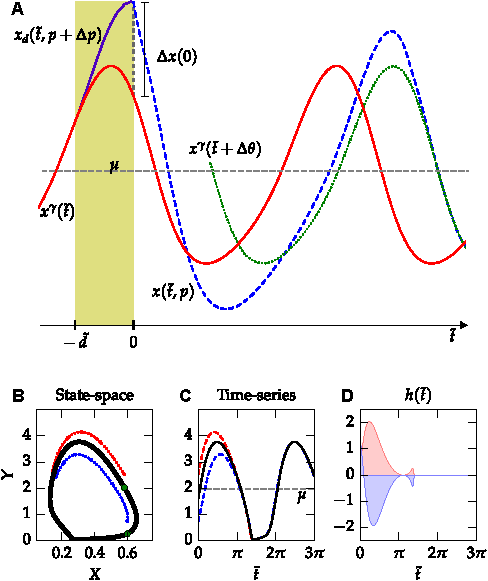
\includegraphics[width=.75\textwidth]{figures/figure_1.pdf}
  %DIFDELCMD < \end{center}
%DIFDELCMD <   %%%
%DIFDELCMD < \caption{%
{%DIFAUXCMD
%DIFDELCMD < {\bfseries %%%
\DIFdelFL{Perturbations to limit cycle models.}%DIFDELCMD < } %%%
\DIFdelFL{(}%DIFDELCMD < {\bfseries %%%
\DIFdelFL{A}%DIFDELCMD < }%%%
\DIFdelFL{)
  Schematic showing trajectories used in the calculation of single-cell phase
  and amplitude change. A perturbation \mbox{%DIFAUXCMD
$x(t,p)$
}%DIFAUXCMD
, blue, from the limit cycle
  solution \mbox{%DIFAUXCMD
$x^\gamma(t,p)$
}%DIFAUXCMD
, red, ultimately returns to the limit cycle with
  a phase shift \mbox{%DIFAUXCMD
$x^\gamma(t + \Delta\theta,p)$
}%DIFAUXCMD
, green. (}%DIFDELCMD < {\bfseries %%%
\DIFdelFL{B-D}%DIFDELCMD < }%%%
\DIFdelFL{) The
  same perturbation applied at two different phases can result in opposite
  amplitude effects. The state-space representation (}%DIFDELCMD < {\bfseries %%%
\DIFdelFL{B}%DIFDELCMD < }%%%
\DIFdelFL{) reveals the
  path both perturbations take to return to the limit cycle. The time-series
  representation (}%DIFDELCMD < {\bfseries %%%
\DIFdelFL{C}%DIFDELCMD < }%%%
\DIFdelFL{) shows how the perturbation in blue results in
  an amplitude decrease, while the one in red results in an amplitude
  increase. (}%DIFDELCMD < {\bfseries %%%
\DIFdelFL{D}%DIFDELCMD < }%%%
\DIFdelFL{) This amplitude change is quantified by integrating
  \mbox{%DIFAUXCMD
$h(\hat{t})$
}%DIFAUXCMD
, the difference in variance from each solution to the limit
  cycle as defined in Eq. \ref{eq:ampchangedefinition}, from \mbox{%DIFAUXCMD
$t=0 \to \infty$
}%DIFAUXCMD
.
  Model adapted from \mbox{%DIFAUXCMD
\cite{Novak2008}
}%DIFAUXCMD
.}}
%DIFAUXCMD
%DIFDELCMD < \end{figure}
%DIFDELCMD < 

%DIFDELCMD < %%%
\DIFdelend Amplitude change for a two-dimensional oscillator is easy to visualize graphically.
In Fig.\DIFaddbegin \DIFadd{~}\DIFaddend 1 B-D, the same state perturbation $\Delta x(0)$ applied at two different phases results in opposite amplitude changes, depending on whether the perturbation shifts the trajectory to the interior of the limit cycle (reduced amplitudes) or to the outside the limit cycle (increased amplitudes).
Trajectories for the second state variable, \DIFdelbegin \DIFdel{\mbox{%DIFAUXCMD
$Y(\hat{t})$
}%DIFAUXCMD
}\DIFdelend \DIFaddbegin \DIFadd{\mbox{%DIFAUXCMD
$Y(\tilde{t})$
}%DIFAUXCMD
}\DIFaddend , and the corresponding integrand for the amplitude change equation, \DIFdelbegin \DIFdel{\mbox{%DIFAUXCMD
$h(\hat{t})$
}%DIFAUXCMD
}\DIFdelend \DIFaddbegin \DIFadd{\mbox{%DIFAUXCMD
$h(\tilde{t})$
}%DIFAUXCMD
}\DIFaddend , demonstrate how this transient change is quantified.


\DIFaddbegin \begin{figure}[tbp]
  \begin{center}
    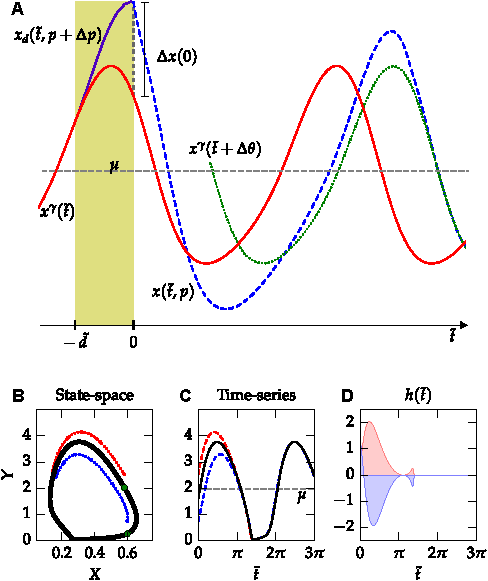
\includegraphics[width=.75\textwidth]{figures/figure_1.pdf}
  \end{center}
  \caption{\DIFaddFL{
{}\bfseries \DIFaddFL{Amplitude metrics at the single-cell level measure transient deviations from the limit cycle}} \DIFaddFL{(}{\bfseries \DIFaddFL{A}}\DIFaddFL{) Schematic showing trajectories used in the calculation of single-cell phase and amplitude change.
A perturbation \mbox{%DIFAUXCMD
$x(\tilde{t},p)$
}%DIFAUXCMD
, blue, from the limit cycle solution \mbox{%DIFAUXCMD
$x^\gamma(\tilde{t},p)$
}%DIFAUXCMD
, red, ultimately returns to the limit cycle with a phase shift \mbox{%DIFAUXCMD
$x^\gamma(\tilde{t} + \Delta\theta,p)$
}%DIFAUXCMD
, green.
(}{\bfseries \DIFaddFL{B-D}}\DIFaddFL{) The same perturbation applied at two different phases can result in opposite amplitude effects.
The state-space representation (}{\bfseries \DIFaddFL{B}}\DIFaddFL{) reveals the path both perturbations take to return to the limit cycle.
The time-series representation (}{\bfseries \DIFaddFL{C}}\DIFaddFL{) shows how the perturbation in blue results in an amplitude decrease, while the one in red results in an amplitude increase.
(}{\bfseries \DIFaddFL{D}}\DIFaddFL{) This amplitude change is quantified by integrating \mbox{%DIFAUXCMD
$h(\tilde{t})$
}%DIFAUXCMD
, the difference in variance from each solution to the limit cycle as defined in Eq.~\ref{eq:ampchangedefinition}, from \mbox{%DIFAUXCMD
$t=0 \to \infty$
}%DIFAUXCMD
.
Here the shaded region indicates the area under the curve, \mbox{%DIFAUXCMD
$\Delta A$
}%DIFAUXCMD
, for the perturbations shown in red and blue.
Model adapted from \mbox{%DIFAUXCMD
\cite{Novak2008}
}%DIFAUXCMD
.
}} \end{figure}


\DIFaddend \subsection*{\DIFdelbegin \DIFdel{Amplitude }\DIFdelend \DIFaddbegin \DIFadd{Single-cell amplitude }\DIFaddend response curves}
Similar to the \DIFdelbegin \DIFdel{phase response curve (PRC)}\DIFdelend \DIFaddbegin \DIFadd{PRC}\DIFaddend , we denote the phase-dependent amplitude change following a perturbation as an amplitude response curve (ARC), using the metric presented in Eq.~\ref{eq:ampchangedefinition}.
In Fig.\DIFaddbegin \DIFadd{~}\DIFaddend 2, we calculate the PRC and ARC for a state perturbation of \DIFdelbegin \DIFdel{3 }\DIFdelend \DIFaddbegin \DIFadd{three }\DIFaddend different strengths.
The weakest perturbation results in type 1 (weak) resetting, in which the phase response curve is continuous, while the strongest perturbation results in type 0 (strong) resetting, in which the \DIFdelbegin \DIFdel{phase response curve }\DIFdelend \DIFaddbegin \DIFadd{PRC }\DIFaddend is discontinuous.
This transition occurs once the state perturbation is strong enough to push the trajectory over the unstable fixed point located at the middle of the limit cycle.
For a perturbation of intermediate strength, at a critical phase the trajectory will be pushed close to the fixed point and take a long time to recover the steady state amplitude.
\DIFdelbegin \DIFdel{This }\DIFdelend \DIFaddbegin \DIFadd{The behavior at this }\DIFaddend singularity point is indicated by a sharp dip in the ARC for this perturbation strength.

\begin{figure}[tbp]
  \begin{center}
    %DIF <  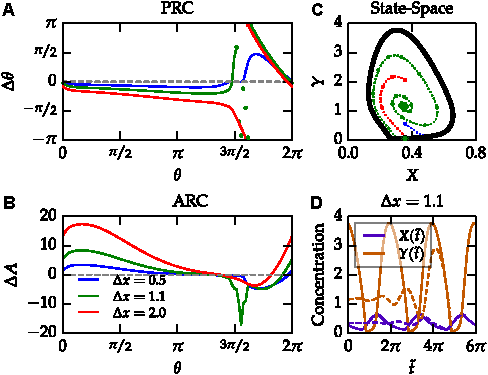
\includegraphics[width=.75\textwidth]{figures/figure_2.pdf}
    \DIFaddbeginFL 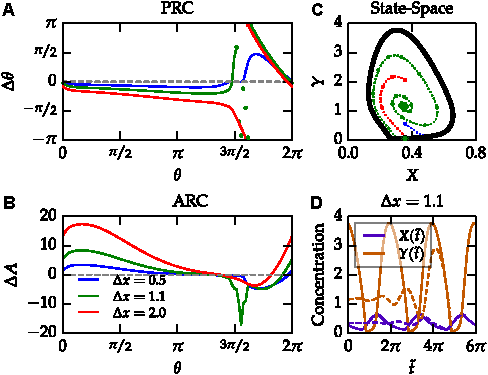
\includegraphics[width=.75\textwidth]{figures/figure_2.pdf}
    \DIFaddendFL \caption{
{\bfseries \DIFdelbeginFL \DIFdelFL{Single cell amplitude and phase response curves.}%DIFDELCMD < } %%%
\DIFdelFL{The
    phase }\DIFdelendFL \DIFaddbeginFL \DIFaddFL{Phase }\DIFaddendFL and amplitude response curves \DIFdelbeginFL \DIFdelFL{determine }\DIFdelendFL \DIFaddbeginFL \DIFaddFL{describe }\DIFaddendFL how a single oscillator will respond to a perturbation.\DIFaddbeginFL }  \DIFaddendFL ({\bfseries A-B}) The phase and amplitude response curves for three perturbations of increasing strengths demonstrate the transition from type 1 phase resetting for a weak stimulus (blue) to type 0 phase resetting from a strong stimulus (red).
({\bfseries C}) The state space representation for the perturbations of varying strengths demonstrate how the trajectories return to the limit cycle.
For the particular perturbation shown in green, the trajectory starts very close to the singularity, and therefore takes a long time to recover.
({\bfseries D}) For an oscillator perturbed to the singularity, a strong amplitude reduction ensues.
Here, the oscillator with an initial phase $\theta \approx \nicefrac{3\pi}{2}$ is perturbed by $\Delta x = 1.1$ at \DIFdelbeginFL \DIFdelFL{\mbox{%DIFAUXCMD
$\hat{t} =
    0$
}%DIFAUXCMD
}\DIFdelendFL \DIFaddbeginFL \DIFaddFL{\mbox{%DIFAUXCMD
$\tilde{t} = 0$
}%DIFAUXCMD
}\DIFaddendFL .
Several cycles are required for normal amplitudes to be restored, corresponding to a dip in the ARC (C, green).}
  \end{center}
\end{figure}

\DIFdelbegin \DIFdel{As with the infinitesimal PRC, it is often desirable to know the derivative
of the oscillation amplitude with respect to a state perturbation or parameter
pulse}\DIFdelend \DIFaddbegin \DIFadd{Infinitesimal versions of response curves are often more general and easier to compute than those that track a specific perturbation strength \mbox{%DIFAUXCMD
\cite{Rand2004}
}%DIFAUXCMD
}\DIFaddend .
We therefore derive an expression for the infinitesimal ARC, defined as:
\DIFdelbegin \begin{displaymath}\DIFdel{
  \frac{dA}{dx} \coloneqq \lim_{\Delta x(0) \to 0} \frac{\Delta
    A\left(x(\hat{t}),\ x^\gamma(\hat{t} + \theta_0 + \Delta\theta)\right)}{\Delta x(0)}
  \label{eq:sARC}
}\end{displaymath}
%DIFAUXCMD
\DIFdelend \DIFaddbegin \begin{equation}\DIFadd{
  \frac{dA}{dx} \coloneqq \lim_{\Delta x(0) \to 0} \frac{\Delta A\left(x(\tilde{t}),\ x^\gamma(\tilde{t} + \theta_0 + \Delta\theta)\right)}{\Delta x(0)} = \int_0^\infty \lim_{\Delta x(0) \to 0} \frac{h(t)}{\Delta x(0)} \; dt
  \label{eq:sARC}
}\end{equation}
\DIFaddend While this quantity could be calculating by using a very small $\Delta x(0)$, it is more accurate and efficient to derive a direct method to calculate Eq.~\ref{eq:sARC} using the ODE sensitivities defined in Eq.~\ref{eq:odesens}.
For simplicity, we define \DIFdelbegin \DIFdel{\mbox{%DIFAUXCMD
$t_\theta = \hat{t} + \theta_0$
}%DIFAUXCMD
}\DIFdelend \DIFaddbegin \DIFadd{\mbox{%DIFAUXCMD
$t_\theta = \tilde{t} + \theta_0$
}%DIFAUXCMD
}\DIFaddend , which allows the time variable for the perturbation to vary from $0 \to \infty$ while tracking the appropriate phase on the limit cycle.
Since $\Delta \theta \to 0$ as $\Delta x(0) \to 0$, we Taylor expand the limit cycle trajectory around $t_\theta$:
\DIFdelbegin \begin{eqnarray*}\DIFdel{
  x^\gamma(t_\theta + \Delta\theta) }&\DIFdel{= x^\gamma(t_\theta) +
  \frac{dx^\gamma(t_\theta)}{d\theta}\Delta\theta + O(\Delta\theta^2)}\\
  &\DIFdel{= x^\gamma(t_\theta) + \hat{f}\left(x^\gamma(t_\theta)\right)\Delta\theta +
  O(\Delta\theta^2)
}\end{eqnarray*}
%DIFAUXCMD
\DIFdel{Simplifying first }\DIFdelend \DIFaddbegin \begin{align}\DIFadd{
  x^\gamma(t_\theta + \Delta\theta) }&\DIFadd{= x^\gamma(t_\theta) +
  \frac{dx^\gamma(t_\theta)}{d\theta}\Delta\theta + O(\Delta\theta^2)}\\
  &\DIFadd{= x^\gamma(t_\theta) + \tilde{f}\left(x^\gamma(t_\theta)\right)\Delta\theta +
  O(\Delta\theta^2)
}\end{align}
\DIFadd{Simplifying }\DIFaddend the integrand in \DIFdelbegin \DIFdel{the numerator of }\DIFdelend Eq.~\ref{eq:sARC}:
\DIFdelbegin \begin{eqnarray*}\DIFdel{
  h(t) }&\DIFdel{= \frac{1}{\Delta x(0)} \left[\left(x^\gamma(t_\theta) +
    \Delta x(\hat{t}) - \mu\right)^2 - \left(x^\gamma(t_\theta +
    \Delta \theta) - \mu\right)^2 \right]}\\
  &\DIFdel{= \frac{1}{\Delta x(0)} \left[\left(x^\gamma(t_\theta) +
    \Delta x(\hat{t}) - \mu\right)^2 - \left(x^\gamma(t_\theta) + \hat{f}\left(x^\gamma(t_\theta)\right)\Delta\theta - \mu\right)^2 \right]}\\
  &\DIFdel{= \frac{1}{\Delta x(0)} \left[\left(\Delta x(\hat{t}) -
    \hat{f}\left(x^\gamma(t_\theta)\right)\Delta\theta\right) \left(\Delta
    x(\hat{t}) + \hat{f}\left(x^\gamma(t_\theta)\right)\Delta\theta +
    2(x^\gamma(t_\theta) - \mu)\right)^2 \right]}\\
    &\DIFdel{= 2\left(\frac{\Delta x(\hat{t})}{\Delta x(0)} -
    \hat{f}\left(x^\gamma(t_\theta)\right)\frac{\Delta\theta}{\Delta
    x(0)}\right) \left(x^\gamma(t_\theta) - \mu\right)
}\end{eqnarray*}
%DIFAUXCMD
\DIFdelend \DIFaddbegin \begin{align}\DIFadd{
  \frac{h(t)}{\Delta x(0)} }&\DIFadd{= \frac{1}{\Delta x(0)} \left[\left(x^\gamma(t_\theta) +
    \Delta x(\tilde{t}) - \mu\right)^2 - \left(x^\gamma(t_\theta +
    \Delta \theta) - \mu\right)^2 \right]}\\
  &\DIFadd{= \frac{1}{\Delta x(0)} \left[\left(x^\gamma(t_\theta) +
    \Delta x(\tilde{t}) - \mu\right)^2 - \left(x^\gamma(t_\theta) + \tilde{f}\left(x^\gamma(t_\theta)\right)\Delta\theta - \mu\right)^2 \right]}\\
  &\DIFadd{= \frac{1}{\Delta x(0)} \left[\left(\Delta x(\tilde{t}) -
    \tilde{f}\left(x^\gamma(t_\theta)\right)\Delta\theta\right) \left(\Delta
    x(\tilde{t}) + \tilde{f}\left(x^\gamma(t_\theta)\right)\Delta\theta +
    2(x^\gamma(t_\theta) - \mu)\right) \right]
}\end{align}
\DIFaddend Taking the limit of this \DIFdelbegin \DIFdel{numerator }\DIFdelend \DIFaddbegin \DIFadd{integrand }\DIFaddend as $\Delta x(0) \to 0$ \DIFdelbegin \DIFdel{allows the
differential terms}\DIFdelend \DIFaddbegin \DIFadd{cancels several differential terms, and allows the remainder }\DIFaddend to be substituted with quantities that can be calculated using ODE sensitivity analysis:
\DIFdelbegin \begin{eqnarray*}\DIFdel{
  \lim_{\Delta x(0) \to 0} h(t) }&\DIFdel{= 2\left(\lim_{\Delta x(0) \to 0}\frac{\Delta
    x(\hat{t})}{\Delta x(0)} -
    \hat{f}\left(x^\gamma(t_\theta)\right)\lim_{\Delta x(0) \to
    0}\frac{\Delta\theta}{\Delta x(0)}\right) \left(x^\gamma(t_\theta) -
    \mu\right)^2}\\
    &\DIFdel{= 2\left(S(\hat{t}) -
    \hat{f}(x^\gamma(t_\theta))\frac{d\theta}{dx}\right)\left(x^\gamma(t_\theta)
    - \mu\right)
}\end{eqnarray*}
%DIFAUXCMD
\DIFdelend \DIFaddbegin \begin{align}\DIFadd{
  \lim_{\Delta x(0) \to 0} \frac{h(t)}{\Delta x(0)} }&\DIFadd{= 2\left(\lim_{\Delta x(0) \to 0}\frac{\Delta x(\tilde{t})}{\Delta x(0)} - \tilde{f}\left(x^\gamma(t_\theta)\right)\lim_{\Delta x(0) \to 0}\frac{\Delta\theta}{\Delta x(0)}\right) \left(x^\gamma(t_\theta) - \mu\right)}\\
  &\DIFadd{= 2\left(S(\tilde{t}) - \tilde{f}(x^\gamma(t_\theta))\frac{d\theta}{dx}\right)\left(x^\gamma(t_\theta) - \mu\right)
  \label{eq:sens_sub}
}\end{align}
\DIFadd{Note that in Eq.~\ref{eq:sens_sub}, \mbox{%DIFAUXCMD
$\nicefrac{d\theta}{dx}$
}%DIFAUXCMD
represents the derivative of \mbox{%DIFAUXCMD
$\Delta\theta$
}%DIFAUXCMD
with respect to the perturbation, and is therefore a scalar quantity.
}\DIFaddend The infinitesimal state-impulse ARC may therefore be calculated directly from the ODE sensitivity matrix and the PRC\DIFdelbegin \DIFdel{:
}\begin{displaymath}\DIFdel{
  \frac{dA}{dx} = \int_0^\infty 2\left(S(\hat{t}) -
    \hat{f}(x^\gamma(t_\theta))\frac{d\theta}{dx}\right)\left(x^\gamma(t_\theta)
    - \mu\right) \; dt
    \label{eq:siARC}
}\end{displaymath}
%DIFAUXCMD
\DIFdelend \DIFaddbegin \DIFadd{, allowing the amplitude change for an infinitesimal perturbation to be calculated exactly and efficiently:
}\begin{equation}\DIFadd{
  \frac{dA}{dx} = \int_0^\infty 2\left(S(\tilde{t}) - \tilde{f}(x^\gamma(t_\theta))\frac{d\theta}{dx}\right)\left(x^\gamma(t_\theta) - \mu\right) \; dt
  \label{eq:siARC}
}\end{equation}
\DIFadd{Here, the first term of the integrand \mbox{%DIFAUXCMD
$(S - \tilde{f}\dot{\theta})$
}%DIFAUXCMD
tracks the distance from the perturbed trajectory to the limit cycle, which decays to zero as \mbox{%DIFAUXCMD
$t \to \infty$
}%DIFAUXCMD
.
The second term \mbox{%DIFAUXCMD
$(x^\gamma - \mu)$
}%DIFAUXCMD
weights this distance by whether or not the deviation occurs above or below the oscillatory mean, yielding negative amplitude changes when the trajectory is perturbed closer to the mean.
}\DIFaddend Just as with the parameter-impulse PRC, the infinitesimal parameter-impulse ARC \DIFdelbegin \DIFdel{:
}\begin{displaymath}\DIFdel{
  \frac{d}{d\hat{t}}\frac{dA}{dp} \coloneqq \lim_{d,\; \Delta p \to 0} 
}\end{displaymath}
%DIFAUXCMD
\DIFdelend \DIFaddbegin \DIFadd{is defined as:
}\begin{equation}\DIFadd{
  \frac{d}{d\tilde{t}}\frac{dA}{dp} \coloneqq \lim_{\tilde{d},\; \Delta p \to 0} \frac{\Delta A}{\tilde{d}\, \Delta p}
}\end{equation}
\DIFadd{and }\DIFaddend may be calculated from the state-impulse version with the following relationship:
\DIFdelbegin \begin{displaymath}\DIFdel{
  \frac{d}{d\hat{t}}\frac{dA}{dp} = \frac{dA}{dx}\frac{d\hat{f}}{dp}
    \label{eq:piARC}
}\end{displaymath}
%DIFAUXCMD
\DIFdelend \DIFaddbegin \begin{equation}\DIFadd{
  \frac{d}{d\tilde{t}}\frac{dA}{dp} = \frac{dA}{dx}\frac{d\tilde{f}}{dp}
    \label{eq:piARC}
}\end{equation}
\DIFadd{As with Eq.~\ref{eq:pPRCequiv}, this equivalency reflects the fact that for a pulse of infinitely short duration, a parameter change is equivalent to changing the state of the system along the direction specified by the Jacobian.
}\DIFaddend Convergence between the methods in Eqs.\DIFaddbegin \DIFadd{~}\DIFaddend \ref{eq:siARC}-\ref{eq:piARC} and finite-difference approaches is shown in Fig.\DIFaddbegin \DIFadd{~}\DIFaddend S1 \DIFaddbegin \DIFadd{in the Supporting Material}\DIFaddend , which demonstrates that the numerically-efficient differential ARCs remain representative even for moderate-strength perturbations.

%DIF <  \section{Population-level Effects}
\DIFdelbegin %DIFDELCMD < 

%DIFDELCMD < %%%
\subsection*{\DIFdel{Phase-diffusion model}}
%DIFAUXCMD
\DIFdel{While single-cell level limit cycle models are often used to understand the
effects of perturbations to clock systems, actual measurements typically come
from a large population of oscillators. The mean bioluminescence signal from
}%DIFDELCMD < {\itshape %%%
\DIFdel{in vitro}%DIFDELCMD < } %%%
\DIFdel{data is determined by a population of cells, each with
their own internal phase. Some modeling studies explicitly consider a
population of oscillators, especially when cell-to-cell coupling or stochastic
effects play an important role \mbox{%DIFAUXCMD
\cite{An2013, To2007}
}%DIFAUXCMD
. However, this approach
complicates the analytical tractability of the system. We show that when the
cells in the population are non-interacting, the population-level dynamics can
be more efficiently understood by combining a single limit cycle model with a
phase probability density model.
}%DIFDELCMD < 

%DIFDELCMD < %%%
\DIFdel{The synchrony of the population is modeled using a probability density function
\mbox{%DIFAUXCMD
$p(\theta, \hat{t})$
}%DIFAUXCMD
which describes the probability of finding an oscillator
at phase \mbox{%DIFAUXCMD
$\theta$
}%DIFAUXCMD
. The usefulness of probability density functions in
describing populations of circadian cells has been shown previously
\mbox{%DIFAUXCMD
\cite{Ukai2007}
}%DIFAUXCMD
. As with all probability density functions,
}\begin{displaymath}\DIFdel{
  \int_0^{2\pi} p(\theta, \hat{t}) \; d\theta = 1
}\end{displaymath}
%DIFAUXCMD
\DIFdel{Since each oscillator in the population follows the dynamics described by
\mbox{%DIFAUXCMD
$x^\gamma(\theta)$
}%DIFAUXCMD
, the population-level expression, \mbox{%DIFAUXCMD
$\bar{x}(\hat{t})$
}%DIFAUXCMD
, is
found by taking the weighted average of the expression level over the current
population:
}\begin{displaymath}\DIFdel{
  \bar{x}(\hat{t}) = \int_0^{2\pi} x^\gamma(\theta) p(\theta, \hat{t}) \;
  d\theta
  \label{eq:xbar}
}\end{displaymath}
%DIFAUXCMD
%DIFDELCMD < 

%DIFDELCMD < %%%
\DIFdel{The shape of \mbox{%DIFAUXCMD
$p(\theta, \hat{t})$
}%DIFAUXCMD
changes as the cells advance in time. Stochastic effects cause the population to gradually desynchronize as slight
cycle-to-cycle variabilities are propagated throughout the population. For a
continuous population of oscillators, these effects are well-described by a
diffusion-convection equation \mbox{%DIFAUXCMD
\cite{Stein1965}
}%DIFAUXCMD
:
}\begin{displaymath}\DIFdel{
  \frac{\partial p}{\partial \hat{t}} = \frac{\partial
  p}{\partial \theta} + d\frac{\partial^2 p}{\partial \theta^2}}\\
  \DIFdel{\label{eq:pde}
}\end{displaymath}
%DIFAUXCMD
\DIFdel{Due to the rescaling of \mbox{%DIFAUXCMD
$t$
}%DIFAUXCMD
, the mean period of the population is \mbox{%DIFAUXCMD
$2\pi$
}%DIFAUXCMD
.
Here, the \mbox{%DIFAUXCMD
$\nicefrac{\partial p}{\partial \theta}$
}%DIFAUXCMD
term, analogous to
convection, describes the mean oscillatory period, while the
\mbox{%DIFAUXCMD
$\nicefrac{\partial^2 p}{\partial \theta^2}$
}%DIFAUXCMD
term describes the diffusion of
phases across \mbox{%DIFAUXCMD
$[0, 2\pi)$
}%DIFAUXCMD
. The phase diffusivity parameter \mbox{%DIFAUXCMD
$d$
}%DIFAUXCMD
(in units of
inverse radians) describes the speed with which the population desynchronizes
and can be fit to experimental data. Equation~\ref{eq:pde} has periodic
boundary conditions, with the phase population at \mbox{%DIFAUXCMD
$t=0$
}%DIFAUXCMD
as the initial
condition:
  \mbox{%DIFAUXCMD
$\phi(\theta)$
}%DIFAUXCMD
:
}\begin{eqnarray*}\DIFdel{
  \text{BCs:}\quad p(0, \hat{t}) }&\DIFdel{= p(2\pi, \hat{t}) }\\
  \DIFdel{\frac{\partial p}{\partial \theta}(0, \hat{t}) }&\DIFdel{= \frac{\partial p}{\partial
  \theta}(2\pi, \hat{t}) }\\
  \DIFdel{\text{IC:}\quad p(\theta, 0) }&\DIFdel{= \phi(\theta)\label{eq:pde_ic}
}\end{eqnarray*}
%DIFAUXCMD
\DIFdel{The solution of Eqs. \ref{eq:pde}-\ref{eq:pde_ic} is well-characterized
\mbox{%DIFAUXCMD
\cite{Chirikjian2009}
}%DIFAUXCMD
, with \mbox{%DIFAUXCMD
$p(\theta, \hat{t})$
}%DIFAUXCMD
evolving in time as the
convolution of the initial conditions with a wrapped normal distribution with
mean \mbox{%DIFAUXCMD
$\hat{t}$
}%DIFAUXCMD
and standard deviation \mbox{%DIFAUXCMD
$\sqrt{2d\hat{t}}$
}%DIFAUXCMD
:
}\begin{displaymath}\DIFdel{
  p(\theta, \hat{t}) = \phi(\theta) * \mathcal{WN}(\theta; \hat{t},
  \sqrt{2\, d\, \hat{t}})
}\end{displaymath}
%DIFAUXCMD
\DIFdel{in which the wrapped normal distribution is defined as:
}\begin{displaymath}\DIFdel{
  {\cal WN}}\DIFdel{(\theta; \mu, \sigma) =
  \frac{1}{\sigma\sqrt{2\pi}}\sum_{k=-\infty}^\infty \exp\left[\frac{-(\theta
  - \mu + 2\pi k)^2}{2\sigma^2}\right]
  \label{eq:wrapped_normal}
}\end{displaymath}
%DIFAUXCMD
\DIFdel{Since the convolution of two normal distributions is also a normal
distribution, it is efficient when possible to describe \mbox{%DIFAUXCMD
$\phi(\theta)$
}%DIFAUXCMD
as a normal distribution with mean \mbox{%DIFAUXCMD
$\mu_0$
}%DIFAUXCMD
and standard deviation \mbox{%DIFAUXCMD
$\sigma_0$
}%DIFAUXCMD
, such
that \mbox{%DIFAUXCMD
$p(\theta, \hat{t})$
}%DIFAUXCMD
can be found analytically through:
}\begin{displaymath}\DIFdel{
  p(\theta, \hat{t}) = \mathcal{WN}(\theta; \mu_0 + \hat{t},
  \sqrt{\sigma_0^2 + 2d^2\hat{t}^2})
}\end{displaymath}
%DIFAUXCMD
%DIFDELCMD < 

%DIFDELCMD < %%%
\DIFdel{This phase-diffusion modelexplains why the gradual damping from experimental
population-level data closely resembles an exponentially damped sinusoid
\mbox{%DIFAUXCMD
\cite{Welsh2004}
}%DIFAUXCMD
.
For the idealized system \mbox{%DIFAUXCMD
$x^\gamma(\theta) = \cos(\theta)$
}%DIFAUXCMD
,
\mbox{%DIFAUXCMD
$\phi(\theta) = \delta(\theta)$
}%DIFAUXCMD
:
}\begin{eqnarray*}\DIFdel{
  \bar{x}(t) }&\DIFdel{= \frac{1}{\sqrt{4\pi dt}}\int_{-\infty}^{\infty}
  \cos(x) \exp\left(-\frac{(x - t)^2}{4dt}\right)\; dx }\\
  &\DIFdel{= \Re\left[\frac{1}{\sqrt{4\pi dt}}\int_{-\infty}^{\infty}
    \exp(ix) \exp\left(-\frac{(x - t)^2}{4dt}\right)\; dx\right] }\\
    &\DIFdel{= \Re\left[e^{(i - d)t}\right]}\\
    &\DIFdel{= e^{-dt} \cos(t) \label{eq:expsin}
}\end{eqnarray*}
%DIFAUXCMD
\DIFdel{Exponential damping and sinusoidal oscillations are still seen with different
limit cycle shapes and initial conditions. The analytical result in Eq.~\ref{eq:expsin} allows us to easily estimate the phase diffusivity
parameter in Eq.~\ref{eq:pde} by simply fitting an exponentially damped
sinusoid to detrended bioluminescence data. 
}%DIFDELCMD < 

%DIFDELCMD < %%%
\DIFdel{In Fig. 3, an initially jagged population density smooths and widens over time
as cells desynchronize, similar to the effects of diffusion. While each cell's
expression level follows the limit cycle, the population amplitude gradually
damps with time as cells with diverse phases are averaged together. This model
closely matches experimental results for cultured fibroblasts, and demonstrates
how limit cycle models can be readily combined with phase-diffusion models.
}%DIFDELCMD < 

%DIFDELCMD < \begin{figure}[tbp]
%DIFDELCMD <   \begin{center}
%DIFDELCMD <     %%%
%DIF <  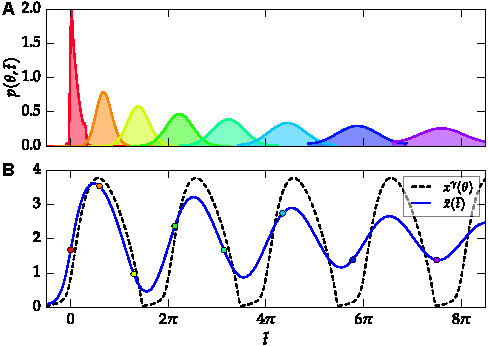
\includegraphics[width=.75\textwidth]{figures/figure_3.pdf}
    %DIFDELCMD < \caption{%
{%DIFAUXCMD
%DIFDELCMD < {\bfseries %%%
\DIFdelFL{Effect of synchrony on population-level amplitude.}%DIFDELCMD < }
%DIFDELCMD <     %%%
\DIFdelFL{(}%DIFDELCMD < {\bfseries %%%
\DIFdelFL{A}%DIFDELCMD < }%%%
\DIFdelFL{) Stochastic fluctuations cause a population of cells to
    gradually desynchronize with time. The phase probability density,
    \mbox{%DIFAUXCMD
$p(\theta, \hat{t})$
}%DIFAUXCMD
, gradually widens as it advances in phase according to
    the mean period. (}%DIFDELCMD < {\bfseries %%%
\DIFdelFL{B}%DIFDELCMD < }%%%
\DIFdelFL{) The mean amplitude from a population of
    oscillators is determined by the probability density function \mbox{%DIFAUXCMD
$p(\theta,
    \hat{t})$
}%DIFAUXCMD
and the oscillator's limit cycle \mbox{%DIFAUXCMD
$x^\gamma(\theta)$
}%DIFAUXCMD
. As time
    passes, population-level rhythms resemble an exponentially damped sinusoid.}}
  %DIFAUXCMD
%DIFDELCMD < \end{center}
%DIFDELCMD < \end{figure}
%DIFDELCMD < 

%DIFDELCMD < %%%
\DIFdelend \subsection*{Population-level response curves}

\DIFdelbegin \DIFdel{A perturbation to a population of oscillators has two simultaneous effects:
first, it perturbs the underlying limit cycle oscillators in a phase-dependent
manner, described by the PRC and ARC of Eqs. \ref{eq:sPRC} and \ref{eq:sARC},
respectively. Secondly, by unevenly shifting the phases of the underlying
oscillators, it changes the phase probability density function. In this
section, we describe how the population-level changes in phase and amplitude
can be found from single-cell level perturbations.
}%DIFDELCMD < 

%DIFDELCMD < %%%
\DIFdelend \DIFaddbegin \DIFadd{We next briefly describe how to calculate the PRC and ARC for a phase-density model.
These approaches are commonly used in understanding phase models \mbox{%DIFAUXCMD
\cite{Kuramoto1984, Ukai2007}
}%DIFAUXCMD
, and are presented here to match previous definitions for single cells.
}\DIFaddend A phase transition curve, $g(\theta) = \theta + \Delta\theta$, maps the phase of an oscillator before perturbation to its phase after the perturbation.
Since individual oscillators are neither created nor destroyed during the perturbation, it is possible - yet numerically difficult - to directly calculate the phase probability distribution following perturbation using the \DIFdelbegin \DIFdel{relation:
}\begin{displaymath}\DIFdel{
  \hat{p}(\theta, \hat{t})\; dg(\theta) = p(\theta, \hat{t})\; d\theta
  \label{eq:pdfinversion}
}\end{displaymath}
%DIFAUXCMD
\DIFdelend \DIFaddbegin \DIFadd{standard change of variables relation:
}\begin{equation}\DIFadd{
  \hat{p}(\theta, \tilde{t})\; dg(\theta) = p(\theta, \tilde{t})\; d\theta
  \label{eq:pdfinversion}
}\end{equation}
\DIFaddend However, it is easier to estimate the mean and standard deviation of the perturbed population \DIFdelbegin \DIFdel{\mbox{%DIFAUXCMD
$\hat{p}(\theta, \hat{t})$
}%DIFAUXCMD
using circular statistics . 
}%DIFDELCMD < 

%DIFDELCMD < %%%
\DIFdelend \DIFaddbegin \DIFadd{\mbox{%DIFAUXCMD
$\hat{p}(\theta, \tilde{t})$
}%DIFAUXCMD
using directional statistics \mbox{%DIFAUXCMD
\cite{Mardia2009}
}%DIFAUXCMD
.
}\DIFaddend A population defined on the unit circle can be described by a complex variable $z = \rho e^{i\bar{\theta}}$, where $\bar{\theta}$ is the mean phase and $\rho$, the synchronization index, is related to the standard deviation of the population.
For $\rho = 1$, the population is clustered about one mean phase, while for $\rho = 0$ the population is evenly balanced across the unit circle.
Complex variables for the population before and after perturbation can be calculated via:
\DIFdelbegin \begin{eqnarray*}\DIFdel{
  z }&\DIFdel{\coloneqq \int_0^{2\pi} e^{i\theta} p(\theta, \hat{t}) \; d\theta \label{eq:zbar}}\\
  \DIFdel{\hat{z} }&\DIFdel{\coloneqq  \int_0^{2\pi} e^{i\theta} \hat{p}(\theta, \hat{t}) \; d\theta =
  \int_0^{2\pi} e^{i g(\theta)} p(\theta, \hat{t}) \; d\theta
  \label{eq:zhat}
}\end{eqnarray*}
%DIFAUXCMD
\DIFdelend \DIFaddbegin \begin{align}\DIFadd{
  z }&\DIFadd{\coloneqq \int_0^{2\pi} e^{i\theta} p(\theta, \tilde{t}) \; d\theta \label{eq:zbar}}\\
  \DIFadd{\hat{z} }&\DIFadd{\coloneqq  \int_0^{2\pi} e^{i\theta} \hat{p}(\theta, \tilde{t}) \; d\theta =
  \int_0^{2\pi} e^{i g(\theta)} p(\theta, \tilde{t}) \; d\theta
  \label{eq:zhat}
}\end{align}
\DIFaddend In Eq.~\ref{eq:zhat}, we avoid calculating the perturbed population explicitly by instead integrating over the new phases at the prior population density function.
Population-level amplitude and phase responses can therefore be calculated by:
\begin{align}
  \Delta \bar{\theta} &= \angle z - \angle \hat{z} \\
  \Delta \rho &= |z| - |\hat{z}|
  \label{eq:popampchange}
\end{align}
Population-level PRCs and ARCs can be tabulated by solving Eqs.\DIFaddbegin \DIFadd{~}\DIFaddend \ref{eq:zbar}-\ref{eq:popampchange} for populations \DIFdelbegin \DIFdel{\mbox{%DIFAUXCMD
$p(\theta, \hat{t})$
}%DIFAUXCMD
}\DIFdelend \DIFaddbegin \DIFadd{\mbox{%DIFAUXCMD
$p(\theta, \tilde{t})$
}%DIFAUXCMD
}\DIFaddend with different mean phases.
\DIFaddbegin \DIFadd{It is important to note that the ARC at the population level strongly depends on the slope of the PRC, as has been shown previously \mbox{%DIFAUXCMD
\cite{Ukai2007}
}%DIFAUXCMD
.
}\DIFaddend 

\DIFdelbegin \DIFdel{In Fig. 4A, we plot single-cell and population-level response curves resulting
from a parameter pulse. In the PRC plot, the single-cell and population curves
are largely similar, in which }\DIFdelend \DIFaddbegin \subsection*{\DIFadd{Population-level mean expression profiles}}

\DIFadd{To efficiently capture }\DIFaddend the population-level \DIFdelbegin \DIFdel{phase change is a slightly
smoothed version of the single-cell response curve.
This smoothing occurs since
the population has an averaging effect on incoming perturbations, with each
cell receiving the input at a slightly different internal phase.
In the ARC
plot, the shape of the }\DIFdelend \DIFaddbegin \DIFadd{effects of bioluminescence experiments, we couple the detailed }\DIFaddend single-cell \DIFdelbegin \DIFdel{and population-based ARC are different,
since they derived from separate mechanisms and describe different changes in the output trajectories}\DIFdelend \DIFaddbegin \DIFadd{ODE model to a phase-density model.
Previous work has used limit cycle models to estimate population-level parameters, such as desynchronization rate, for phase-only models \mbox{%DIFAUXCMD
\cite{Rougemont2007}
}%DIFAUXCMD
.
In this study, we use an ODE model to calculate the response to a perturbation at each phase, and subsequently take the weighted average of these responses according to the phases of the cells in the population}\DIFaddend .

\DIFdelbegin \DIFdel{Using these response curves, we demonstrate characteristic features of
amplitude change mediated at the single-cell and }\DIFdelend \DIFaddbegin \DIFadd{Assuming each oscillator in the population follows the dynamics described by \mbox{%DIFAUXCMD
$x^\gamma(\theta)$
}%DIFAUXCMD
, the unperturbed mean }\DIFaddend population-level \DIFdelbegin \DIFdel{. In Fig. 4B
the perturbation does not cause a significant change in phase or populationsynchrony, yet strongly reduces single-cell amplitudes. The resulting
}\DIFdelend \DIFaddbegin \DIFadd{expression, \mbox{%DIFAUXCMD
$\bar{x}(\tilde{t})$
}%DIFAUXCMD
, can be found by taking the weighted average of the expression level over the current population:
}\begin{equation}\DIFadd{
  \bar{x}(\tilde{t}) = \int_0^{2\pi} x^\gamma(\theta) p(\theta, \tilde{t}) \;
  d\theta
  \label{eq:xbar}
}\end{equation}

\DIFadd{Phase-diffusion models can explain why the gradual damping from experimental }\DIFaddend population-level \DIFdelbegin \DIFdel{trajectory appears damped for the first cycle, until the oscillators return to the limit cycle and normal amplitudes are restored. In
Fig. 4C the perturbation reduces the population synchrony while increasing
single-cell amplitudes, yielding amplitudes that are transiently increased
before the population settles to a lower-amplitude, desynchronized trajectory.
These features allow us to distinguish between these two sources of amplitude
change without explicitly recording single-cell amplitudes: amplitude change
induced at the }\DIFdelend \DIFaddbegin \DIFadd{data closely resembles an exponentially damped sinusoid, a result that has been shown experimentally \mbox{%DIFAUXCMD
\cite{Welsh2004}
}%DIFAUXCMD
and computationally \mbox{%DIFAUXCMD
\cite{Rougemont2007}
}%DIFAUXCMD
.
Our method similarly demonstrates exponential decay: for the idealized system \mbox{%DIFAUXCMD
$x^\gamma(\theta) = \cos(\theta)$
}%DIFAUXCMD
starting from a synchronized state:
}\begin{align}\DIFadd{
  \bar{x}(\tilde{t}) }&\DIFadd{= \frac{1}{\sqrt{4\pi d\tilde{t}}}\int_{-\infty}^{\infty}
  \cos(x) \exp\left(-\frac{(x - \tilde{t})^2}{4d\tilde{t}}\right)\; dx }\\
  &\DIFadd{= \Re\left[\frac{1}{\sqrt{4\pi d\tilde{t}}}\int_{-\infty}^{\infty}
    \exp(ix) \exp\left(-\frac{(x - \tilde{t})^2}{4d\tilde{t}}\right)\; dx\right] }\\
    &\DIFadd{= \Re\left[e^{(i - d)\tilde{t}}\right]}\\
    &\DIFadd{= e^{-d\tilde{t}} \cos(\tilde{t}) \label{eq:expsin}
}\end{align}
\DIFadd{Due to the smoothing effect of phase diffusion, higher frequency sinusoidal components of the limit cycle are damped faster than lower frequency components, resulting in an exponentially decaying sinusoids even for limit cycles that are not sinusoidal in sufficiently disperse populations.
The analytical result in Eq.~\ref{eq:expsin} allows us to easily estimate the phase diffusivity parameter in Eq.~\ref{eq:pde} by simply fitting an exponentially damped sinusoid to detrended bioluminescence data.
}


\DIFadd{Using our continuous approximation to }\DIFaddend population-level \DIFdelbegin \DIFdel{will follow a consistent decaying sinusoid ,
while a change induced at the single-cell level will deviate from this
exponential decay.
Additionally, these results underscore the importance in
considering both single-cell and population-mediated amplitude change in
predicting }\DIFdelend \DIFaddbegin \DIFadd{dynamics, we demonstrate an example unperturbed trajectory using Model 1 (adapted from \mbox{%DIFAUXCMD
\cite{Novak2008}
}%DIFAUXCMD
, see Supporting Material).
In Fig.~3, an initially jagged population density smooths and widens over time as cells desynchronize, similar to }\DIFaddend the effects of \DIFdelbegin \DIFdel{daily stimuli on clock amplitudes}\DIFdelend \DIFaddbegin \DIFadd{diffusion.
While each cell's expression level follows the limit cycle, the population amplitude gradually damps with time as cells with diverse phases are averaged together}\DIFaddend .


\begin{figure}[tbp]
  \begin{center}
    %DIF <  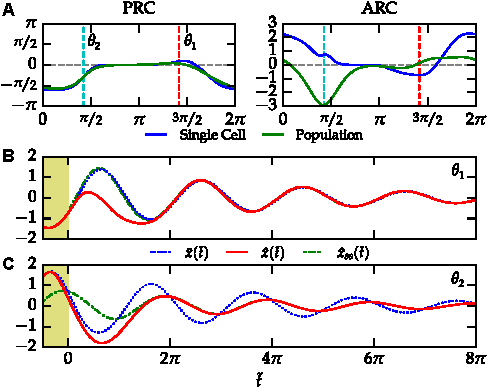
\includegraphics[width=.75\textwidth]{figures/figure_4.pdf}
    \DIFaddbeginFL 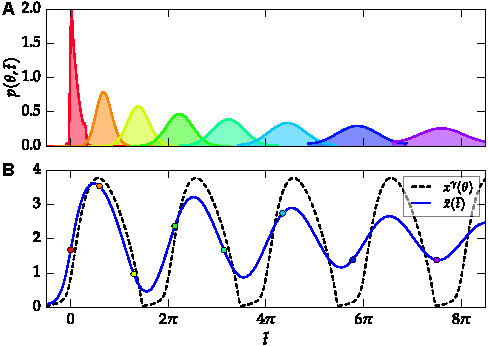
\includegraphics[width=.75\textwidth]{figures/figure_3.pdf}
    \DIFaddendFL \caption{
{\bfseries \DIFdelbeginFL \DIFdelFL{Response curves for a population of oscillators.}%DIFDELCMD < } %%%
\DIFdelFL{A
    temporary parameter change, which induces both a phase response and
    }\DIFdelendFL \DIFaddbeginFL \DIFaddFL{Synchrony affects population-level }\DIFaddendFL amplitude\DIFdelbeginFL \DIFdelFL{change, is applied to a population of oscillators}\DIFdelendFL .\DIFaddbeginFL }
\DIFaddendFL ({\bfseries A}) \DIFdelbeginFL \DIFdelFL{The phase response curves are shown for both the single limit cycle
    oscillator and }\DIFdelendFL \DIFaddbeginFL \DIFaddFL{Stochastic fluctuations cause a }\DIFaddendFL population \DIFdelbeginFL \DIFdelFL{average, left.  The population-level amplitude
    response curve is shown together with the single-cell amplitude response,
    with both curves normalized }\DIFdelendFL \DIFaddbeginFL \DIFaddFL{of cells }\DIFaddendFL to \DIFdelbeginFL \DIFdelFL{\mbox{%DIFAUXCMD
$\sigma=1$
}%DIFAUXCMD
. (}%DIFDELCMD < {\bfseries %%%
\DIFdelFL{B-C}%DIFDELCMD < }%%%
\DIFdelFL{)
    Population-level rhythms, \mbox{%DIFAUXCMD
$\hat{x}(\hat{t})$
}%DIFAUXCMD
resulting from perturbations
    given at the indicated phases in A (red and cyan lines, respectively)}\DIFdelendFL \DIFaddbeginFL \DIFaddFL{gradually desynchronize with time}\DIFaddendFL .
The \DIFdelbeginFL \DIFdelFL{population transitions from the unperturbed population}\DIFdelendFL \DIFaddbeginFL \DIFaddFL{phase probability density}\DIFaddendFL , \DIFdelbeginFL \DIFdelFL{\mbox{%DIFAUXCMD
$\bar{x}(\hat{t})$
}%DIFAUXCMD
}\DIFdelendFL \DIFaddbeginFL \DIFaddFL{\mbox{%DIFAUXCMD
$p(\theta, \tilde{t})$
}%DIFAUXCMD
}\DIFaddendFL , \DIFaddbeginFL \DIFaddFL{gradually widens as it advances in phase according }\DIFaddendFL to the \DIFdelbeginFL \DIFdelFL{steady-state perturbed population, \mbox{%DIFAUXCMD
$\hat{x}_{ss}(\hat{t})$
}%DIFAUXCMD
}\DIFdelendFL \DIFaddbeginFL \DIFaddFL{mean period}\DIFaddendFL .
({\bfseries B}) \DIFdelbeginFL \DIFdelFL{A perturbation at this phase yields a transient }\DIFdelendFL \DIFaddbeginFL \DIFaddFL{The mean }\DIFaddendFL amplitude \DIFdelbeginFL \DIFdelFL{reduction resulting }\DIFdelendFL from \DIFdelbeginFL \DIFdelFL{perturbations at the single-cell level, however,
    there is little change in population synchrony.  Population-level rhythms
    are therefore transiently damped before regaining normal amplitudes.
    (}%DIFDELCMD < {\bfseries %%%
\DIFdelFL{C}%DIFDELCMD < }%%%
\DIFdelFL{) Oscillators are desynchronized, but with }\DIFdelendFL a \DIFdelbeginFL \DIFdelFL{transient
    increase in }\DIFdelendFL \DIFaddbeginFL \DIFaddFL{population of oscillators is determined by the probability density function \mbox{%DIFAUXCMD
$p(\theta, \tilde{t})$
}%DIFAUXCMD
and the oscillator's }\DIFaddendFL limit cycle \DIFdelbeginFL \DIFdelFL{amplitude}\DIFdelendFL \DIFaddbeginFL \DIFaddFL{\mbox{%DIFAUXCMD
$x^\gamma(\theta)$
}%DIFAUXCMD
}\DIFaddendFL .
\DIFdelbeginFL \DIFdelFL{It therefore takes some }\DIFdelendFL \DIFaddbeginFL \DIFaddFL{As }\DIFaddendFL time \DIFdelbeginFL \DIFdelFL{before the
    amplitude reduction from desynchrony is realized}\DIFdelendFL \DIFaddbeginFL \DIFaddFL{passes, population-level rhythms resemble an exponentially damped sinusoid}\DIFaddendFL .}
  \end{center}
\end{figure}

\DIFdelbegin \subsection*{\DIFdel{Calculation of perturbed population trajectories}}
%DIFAUXCMD
\DIFdelend Next we describe how to calculate \DIFdelbegin \DIFdel{the perturbed population trajectories, such
as those shown in Fig. 4 B and C. The unperturbed trajectory,
\mbox{%DIFAUXCMD
$\bar{x}(\hat{t})$
}%DIFAUXCMD
, was previously defined in Eq.~\ref{eq:xbar}}\DIFdelend \DIFaddbegin \DIFadd{population-level mean expression following a perturbation}\DIFaddend .
The perturbed trajectory \DIFdelbegin \DIFdel{\mbox{%DIFAUXCMD
$\hat{x}(\hat{t})$
}%DIFAUXCMD
}\DIFdelend \DIFaddbegin \DIFadd{\mbox{%DIFAUXCMD
$\hat{x}(\tilde{t})$
}%DIFAUXCMD
}\DIFaddend can be decomposed into contributions from two sources.
First, for long times after the perturbation, each individual oscillator will have returned to the limit cycle $x^\gamma(\theta)$, but with a new population density \DIFdelbegin \DIFdel{\mbox{%DIFAUXCMD
$\hat{p}(\theta, \hat{t})$
}%DIFAUXCMD
}\DIFdelend \DIFaddbegin \DIFadd{\mbox{%DIFAUXCMD
$\hat{p}(\theta, \tilde{t})$
}%DIFAUXCMD
}\DIFaddend .
This steady-state perturbed trajectory \DIFdelbegin \DIFdel{\mbox{%DIFAUXCMD
$\hat{x}_{ss}(\hat{t})$
}%DIFAUXCMD
}\DIFdelend \DIFaddbegin \DIFadd{\mbox{%DIFAUXCMD
$\hat{x}_{ss}(\tilde{t})$
}%DIFAUXCMD
}\DIFaddend can be found by:
\DIFdelbegin \begin{displaymath}\DIFdel{
  \hat{x}_{ss}(\hat{t}) = \int_0^{2\pi} x^\gamma(\theta) \hat{p}(\theta,
  \hat{t}) \; d\theta
  \label{eq:xhatss}
}\end{displaymath}
%DIFAUXCMD
\DIFdelend \DIFaddbegin \begin{equation}\DIFadd{
  \hat{x}_{ss}(\tilde{t}) = \int_0^{2\pi} x^\gamma(\theta) \hat{p}(\theta, \tilde{t}) \; d\theta
  \label{eq:xhatss}
}\end{equation}
\DIFaddend For very long times following perturbation, the new phase probability density could be approximated using the initial mean and standard deviation found through Eq.~\ref{eq:zhat}, as jagged profiles in the population density will eventually smooth to a normal distribution.
However, for shorter times following perturbation, \DIFdelbegin \DIFdel{\mbox{%DIFAUXCMD
$\hat{p}(\theta, \hat{t})$
}%DIFAUXCMD
}\DIFdelend \DIFaddbegin \DIFadd{\mbox{%DIFAUXCMD
$\hat{p}(\theta, \tilde{t})$
}%DIFAUXCMD
}\DIFaddend must be calculated numerically.

The second contribution to the perturbed population trajectory comes from deviations from \DIFdelbegin \DIFdel{limit-cycle }\DIFdelend \DIFaddbegin \DIFadd{limit cycle }\DIFaddend oscillations in each cell.
\DIFdelbegin \DIFdel{To }\DIFdelend \DIFaddbegin \DIFadd{We }\DIFaddend calculate the population-level effect of these deviations \DIFdelbegin \DIFdel{, we }\DIFdelend \DIFaddbegin \DIFadd{by averaging over the deviations that occur at each phase.
We }\DIFaddend define the deviation trajectory \DIFdelbegin \DIFdel{\mbox{%DIFAUXCMD
$\delta x(\theta, \hat{t})$
}%DIFAUXCMD
}\DIFdelend \DIFaddbegin \DIFadd{\mbox{%DIFAUXCMD
$\delta x(\theta, \tilde{t})$
}%DIFAUXCMD
}\DIFaddend for each phase as the distance between the \DIFdelbegin \DIFdel{single-cell }\DIFdelend perturbed trajectory and the phase-adjusted reference:
\DIFdelbegin \begin{eqnarray*}\DIFdel{
  \delta x(\theta_0, \hat{t}) }&\DIFdel{\coloneqq x(\hat{t}) - x^\gamma(\hat{t} + \theta_0 +
  \Delta \theta) }\\
 \DIFdel{\therefore\; \lim_{\hat{t} \to \infty} \delta x(\theta, \hat{t}) }&\DIFdel{= 0
}\end{eqnarray*}
%DIFAUXCMD
\DIFdel{Since the deviation trajectories are calculated at each initial phase, they are
averaged by the initial, rather than final, phase probabilities in the equation
for \mbox{%DIFAUXCMD
$\hat{x}(\hat{t})$
}%DIFAUXCMD
:
}\begin{displaymath}\DIFdel{
  \hat{x}(\hat{t}) = \int_0^{2\pi} x^\gamma(\theta)\hat{p}(\theta, \hat{t})
  + \delta x(\theta, \hat{t})p(\theta, \hat{t}) \; d\theta
}\end{displaymath}
%DIFAUXCMD
%DIFDELCMD < 

%DIFDELCMD < %%%
\DIFdelend \DIFaddbegin \begin{align}\DIFadd{
  \delta x(\theta_0, \tilde{t}) }&\DIFadd{\coloneqq x(\tilde{t}) - x^\gamma(\tilde{t} + \theta_0 + \Delta \theta) }\\
  \DIFadd{\therefore\; \lim_{\tilde{t} \to \infty} \delta x(\theta, \tilde{t}) }&\DIFadd{= 0
}\end{align}
\DIFadd{Since the perturbed trajectory ultimately converges with the phase-adjusted reference, deviations will converge to zero.
Since the phase change, \mbox{%DIFAUXCMD
$\Delta\theta$
}%DIFAUXCMD
, associated with a perturbation at each phase is likely not known prior to calculating the perturbed trajectory, it is difficult to tabulate deviation trajectories associated with each final phase, \mbox{%DIFAUXCMD
$\theta_0 + \Delta\theta$
}%DIFAUXCMD
.
It is therefore more straightforward to find the average effect of single-cell perturbations at the population level by weighting the deviations by the phase density function prior to perturbation.
The population-level response to a perturbation, \mbox{%DIFAUXCMD
$\hat{x}(\tilde{t})$
}%DIFAUXCMD
, is therefore defined as:
}\begin{equation}\DIFadd{
  \hat{x}(\tilde{t}) = \int_0^{2\pi} x^\gamma(\theta)\hat{p}(\theta, \tilde{t}) + \delta x(\theta, \tilde{t})p(\theta, \tilde{t}) \; d\theta
  \label{eq:xhat}
}\end{equation}
\DIFadd{Here the first term is equivalent to \mbox{%DIFAUXCMD
$\hat{x}_{ss}(\tilde{t})$
}%DIFAUXCMD
, the steady-state perturbed trajectory, while the second term decays to zero as individual oscillators return to their steady-state amplitude.
}\DIFaddend The accuracy of the continuous phase-diffusion model was tested by explicitly simulating a \DIFaddbegin \DIFadd{perturbation to a }\DIFaddend population of 225 uncoupled oscillators using a stochastic simulation algorithm \DIFdelbegin \DIFdel{\mbox{%DIFAUXCMD
\cite{Sanft2011a}
}%DIFAUXCMD
}\DIFdelend \DIFaddbegin \DIFadd{\mbox{%DIFAUXCMD
\cite{Gillespie1977, Sanft2011a}
}%DIFAUXCMD
}\DIFaddend .
Good agreement between the stochastic population and continuous approximation was shown in phase shift, single-cell level amplitude change, and alteration of population synchrony (Fig.\DIFaddbegin \DIFadd{~}\DIFaddend S2, Movies S1 \& S2).
These results indicate the use of a continuous probability function is justified in the case of \DIFdelbegin \DIFdel{biological }\DIFdelend \DIFaddbegin \DIFadd{cultured cellular reporter }\DIFaddend systems, which may contain up to $10^5$ individual cells per culture \cite{Welsh2004}.
\DIFaddbegin \DIFadd{In addition, the method was verified by similar simulations using the Oregonator \mbox{%DIFAUXCMD
\cite{Field1974}
}%DIFAUXCMD
, a model containing only mass-action terms, and a detailed mechanistic model of circadian rhythms \mbox{%DIFAUXCMD
\cite{Hirota2012}
}%DIFAUXCMD
at a variety of phase timings (Fig.~S3).
The continuous approximation is therefore able to capture the population-level dynamics of a wide variety of limit cycle models and perturbations.
}

\DIFadd{We next demonstrate the usefulness of single-cell and population level ARCs in predicting the mean response of a population.
Using a detailed single-cell model (Model 2), we calculate the response of the system, specifically the average CRY2 protein expression level, to a temporary increase in }{\itshape \DIFadd{Per}} \DIFadd{transcription rate.
In Fig.~4A, we plot the resulting single-cell and population-level response curves.
In this case, the population-level phase change is a slightly smoothed version of the single-cell PRC, since the population has an averaging effect on incoming perturbations with each cell receiving the input at a slightly different internal phase.
This smoothing follows from the consistent definition of phase between the single-cell and population level.
In the ARC plot, however, the shape of the single-cell and population-based ARC are different, since they describe different types of changes (finite vs.}\ \DIFadd{sustained) in the output trajectories.
}

\DIFadd{Using these response curves, we demonstrate characteristic features of amplitude change mediated at the single-cell and population-level.
In Fig.~4B the perturbation at \mbox{%DIFAUXCMD
$\theta_1$
}%DIFAUXCMD
does not cause a significant change in phase or population synchrony, yet strongly reduces single-cell amplitudes.
The resulting population-level trajectory appears damped for the first cycle, until the oscillators within the population return to the limit cycle and normal amplitudes are restored.
In Fig.~4C the perturbation at \mbox{%DIFAUXCMD
$\theta_2$
}%DIFAUXCMD
reduces population synchrony while increasing single-cell amplitudes, yielding amplitudes that are transiently increased before the population settles to a lower-amplitude, desynchronized trajectory.
}

\DIFadd{These examples demonstrate the qualitative differences between amplitude change mediated at the single-cell and population level.
Their characteristic features allow us to distinguish between these two sources of amplitude change without explicitly recording single-cell amplitudes: amplitude change induced at the population-level will be sustained, but may be masked in the short term by changes to single-cell level amplitudes.
Similarly, a change induced at the single-cell level will be evident only at short time-scales.
These results underscore the importance in considering both single-cell and population-mediated amplitude change in predicting the effects of daily stimuli on clock amplitudes.
}

\begin{figure}[tbp]
  \begin{center}
    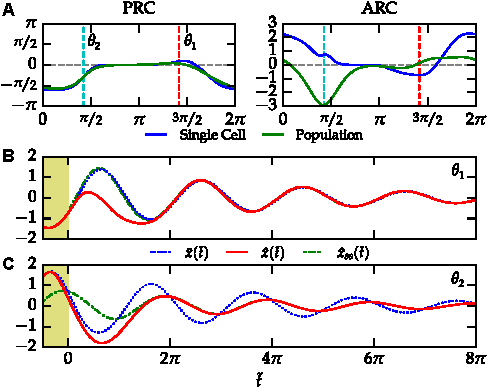
\includegraphics[width=.75\textwidth]{figures/figure_4.pdf}
    \caption{\DIFaddFL{
{}\bfseries \DIFaddFL{Response curves describe different types of amplitude change.}}
\DIFaddFL{A population of cells is simulated using a detailed model of circadian rhythms (Model 2).
Each cell in the population is subjected to a \mbox{%DIFAUXCMD
$20\%$
}%DIFAUXCMD
increase in the \mbox{%DIFAUXCMD
$\mathit{vtp}$
}%DIFAUXCMD
parameter (}{\itshape \DIFaddFL{Per}} \DIFaddFL{transcription rate) for \mbox{%DIFAUXCMD
$d=\nicefrac{\pi}{2}$
}%DIFAUXCMD
, inducing both a phase and amplitude change.
(}{\bfseries \DIFaddFL{A}}\DIFaddFL{) The phase response curves are shown for both the single limit cycle oscillator and population average, left.
The population-level ARC is shown together with the single-cell amplitude response, with both curves normalized to \mbox{%DIFAUXCMD
$\sigma=1$
}%DIFAUXCMD
.
(}{\bfseries \DIFaddFL{B-C}}\DIFaddFL{) Population-level rhythms, \mbox{%DIFAUXCMD
$\hat{x}(\tilde{t})$
}%DIFAUXCMD
resulting from perturbations given at the indicated phases in A (red and cyan lines, respectively).
The population transitions from the unperturbed population, \mbox{%DIFAUXCMD
$\bar{x}(\tilde{t})$
}%DIFAUXCMD
, to the steady-state perturbed population, \mbox{%DIFAUXCMD
$\hat{x}_{ss}(\tilde{t})$
}%DIFAUXCMD
.
(}{\bfseries \DIFaddFL{B}}\DIFaddFL{) A perturbation at this phase yields a transient amplitude reduction resulting from perturbations at the single-cell level, however, there is little change in population synchrony.
Population-level rhythms are therefore transiently damped before regaining normal amplitudes.
(}{\bfseries \DIFaddFL{C}}\DIFaddFL{) Oscillators are desynchronized, but with a transient increase in limit cycle amplitude.
It therefore takes some time before the amplitude reduction from desynchrony is realized.}}
  \end{center}
\end{figure}
\DIFaddend 

%DIF <  \section{Application to Experimental Data}
\subsection*{Application to Experimental Data}
\DIFdelbegin \DIFdel{We finish by demonstrating how }\DIFdelend \DIFaddbegin 

\DIFadd{We conclude by using }\DIFaddend the proposed modeling framework \DIFdelbegin \DIFdel{is able to accurately reproduce bioluminescence experiments.
}\DIFdelend \DIFaddbegin \DIFadd{to reconcile two experimental studies that measured the effect of light on the circadian amplitude of photosensitive fibroblast cells \mbox{%DIFAUXCMD
\cite{Ukai2007, Pulivarthy2007}
}%DIFAUXCMD
.
Both studies sought to determine the main factor of amplitude reduction following a transient light pulse, in which either desynchrony alone \mbox{%DIFAUXCMD
\cite{Ukai2007}
}%DIFAUXCMD
or a combination of single-cell amplitude reduction and desynchrony \mbox{%DIFAUXCMD
\cite{Pulivarthy2007}
}%DIFAUXCMD
was identified as the dominant factor.
}

\DIFaddend Data on the response of melanopsin-responsive and control NIH3T3 mouse fibroblasts cells is shown in Fig.\DIFdelbegin \DIFdel{5A \mbox{%DIFAUXCMD
\cite{Ukai2007}
}%DIFAUXCMD
.
}\DIFdelend \DIFaddbegin \DIFadd{~5B \mbox{%DIFAUXCMD
\cite{Ukai2007}
}%DIFAUXCMD
.
The experimental data is de-noised using a discrete wavelet transform \mbox{%DIFAUXCMD
\cite{Leise2011}
}%DIFAUXCMD
.
}\DIFaddend In the experiment, a light pulse is given to desynchronize a colony of cells, resulting in drastically reduced amplitudes.
A second (longer) light pulse subsequently re-synchronizes the population, resulting in increased amplitudes.
\DIFdelbegin %DIFDELCMD < 

%DIFDELCMD < %%%
\DIFdelend To capture this phenomenon {\itshape in silico}, we used a recent model of the core circadian feedback circuit \cite{Hirota2012}.
\DIFdelbegin \DIFdel{We }\DIFdelend \DIFaddbegin \DIFadd{In order to find parameters for the phase density function, we }\DIFaddend assumed an initial phase population with $\sigma = 0.1$ and calculated a phase diffusivity parameter $d = 0.104$ from the experimental control trajectory.
\DIFdelbegin \DIFdel{From these
values, desynchronization ARCs revealed which parameters had the greatest
effect on population synchrony.
The }\DIFdelend \DIFaddbegin 

\DIFadd{The next step in capturing the experimental data was finding a perturbation capable of desynchronizing the system.
To find such a perturbation, we calculated population-level ARCs at several different knockdown strengths for each parameter in the model.
We selected the }\DIFaddend degradation rate of {\itshape Per} mRNA \DIFdelbegin \DIFdel{was
chosen at a suitable parameter}\DIFdelend \DIFaddbegin \DIFadd{from the feasible parameters}\DIFaddend , due to \DIFdelbegin \DIFdel{its ability to desynchronize the
population and }\DIFdelend PER's known induction by CREB following photo-perturbation \cite{Tischkau2003}.
The parameter was reduced by $28.5\%$ during the light pulses, a value fit to maximize light-induced desynchrony.
The output variable, PER2-luciferase in the experimental system, was chosen to be represented by {\itshape Cry1} mRNA - an E box activated gene \DIFdelbegin \DIFdel{which }\DIFdelend \DIFaddbegin \DIFadd{that }\DIFaddend is buffered from the direct effects of the parameter perturbation.
\DIFaddbegin \DIFadd{The single-cell and population-level response curves for this parameter choice are shown in Fig.~5A, which demonstrates the strong desynchronization that occurs at \mbox{%DIFAUXCMD
$\theta\approx\nicefrac{\pi}{4}$
}%DIFAUXCMD
.
Since the reporter used in the experimental system likely has a phase lag from the corresponding mRNA, we did not try to match the initial phase of the simulation to experiment.
Instead, the initial phase of simulation was chosen such that the first pulse occurred when the system was at the phase that corresponded with the minimum of the population-level ARC.
}\DIFaddend 


\begin{figure}[tbp]
  \begin{center}
    %DIF <  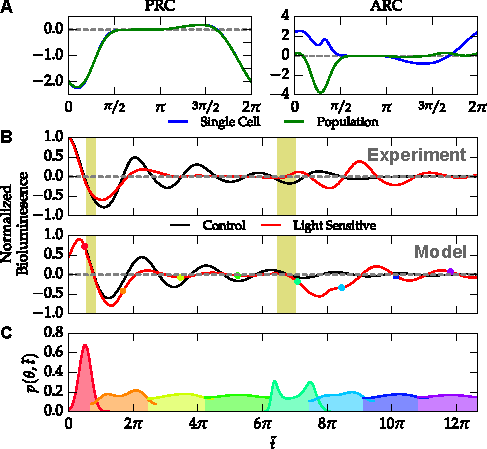
\includegraphics[width=.75\textwidth]{figures/figure_5.pdf}
    \DIFaddbeginFL 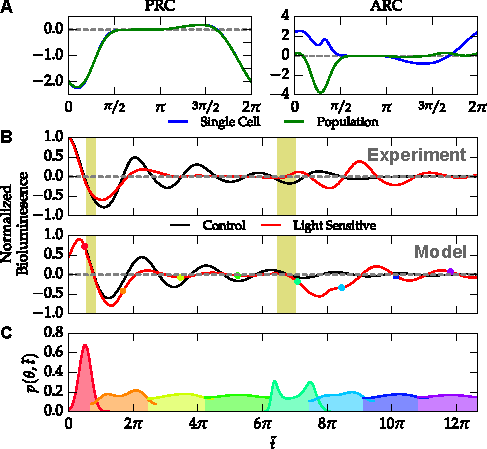
\includegraphics[width=.75\textwidth]{figures/figure_5.pdf}
    \DIFaddendFL \caption{
{\bfseries \DIFdelbeginFL \DIFdelFL{Probability-based population models accurately
    reproduce }\DIFdelendFL \DIFaddbeginFL \DIFaddFL{Method allows direct comparison between model results and }\DIFaddendFL experimental \DIFdelbeginFL \DIFdelFL{perturbations}\DIFdelendFL \DIFaddbeginFL \DIFaddFL{bioluminescence profiles}\DIFaddendFL .} 
({\bfseries A}) \DIFaddbeginFL \DIFaddFL{Response curves for the parameter perturbation used to model the first light pulse in (B).
The initial phase of the system is chosen to coincide with the strong dip in the population-level ARC (left).
(}{\bfseries \DIFaddFL{B}}\DIFaddFL{) }\DIFaddendFL De-noised bioluminescence data from Ukai {\itshape et al.} 2007 (top) demonstrates population-level amplitude change resulting from two light pulses \cite{Ukai2007}.
\DIFdelbeginFL \DIFdelFL{The }\DIFdelendFL \DIFaddbeginFL \DIFaddFL{Circadian oscillations are suppressed by the }\DIFaddendFL first \DIFaddbeginFL \DIFaddFL{light }\DIFaddendFL pulse \DIFdelbeginFL \DIFdelFL{desynchronizes the system, while
    }\DIFdelendFL \DIFaddbeginFL \DIFaddFL{and rescued by }\DIFaddendFL the second\DIFdelbeginFL \DIFdelFL{resynchronizes}\DIFdelendFL .
These perturbations were reproduced {\itshape in silico} (bottom) using the model from Hirota {\itshape et al.} 2012.
The experimental results are qualitatively captured by the model, demonstrating the suitability of the \DIFdelbeginFL \DIFdelFL{population model }\DIFdelendFL \DIFaddbeginFL \DIFaddFL{method }\DIFaddendFL in capturing bioluminescence experiments.
\DIFaddbeginFL \DIFaddFL{The relative amplitude of the model equations has been scaled to match that of the normalized bioluminescence profiles.
}\DIFaddendFL ({\bfseries \DIFdelbeginFL \DIFdelFL{B}\DIFdelendFL \DIFaddbeginFL \DIFaddFL{C}\DIFaddendFL }) Example probability density functions for the model trajectory shown in \DIFaddbeginFL \DIFaddFL{(}\DIFaddendFL A\DIFaddbeginFL \DIFaddFL{)}\DIFaddendFL .
 The initial population (red) is effectively desynchronized \DIFaddbeginFL \DIFaddFL{(orange) }\DIFaddendFL following the first light pulse\DIFdelbeginFL \DIFdelFL{(orange)}\DIFdelendFL .
Following the second light pulse, stronger peaks are seen (teal), which gradually damp as time evolves.} \end{center}
\end{figure}

\DIFdelbegin \DIFdel{The model-predicted }\DIFdelend \DIFaddbegin \DIFadd{Population-level trajectories were found by solving for the resulting limit cycle trajectories at every phase, and subsequently finding the weighted average of these trajectories according the phase density (as described in Eqs.~\ref{eq:xbar} and \ref{eq:xhat}).
The simulated }\DIFaddend control and perturbed trajectories, Fig.\DIFdelbegin \DIFdel{5A}\DIFdelend \DIFaddbegin \DIFadd{~5B}\DIFaddend , closely match the experimental results, in which the model captures both the phase shifts and amplitude modulation of the light pulses.
The phase probability density function for the light-sensitive model trajectory is shown in Fig.\DIFdelbegin \DIFdel{4B }\DIFdelend \DIFaddbegin \DIFadd{~5C }\DIFaddend for several representative time points.
Changes to the synchronization of the population from each perturbation are readily apparent, \DIFdelbegin \DIFdel{and }\DIFdelend \DIFaddbegin \DIFadd{with both perturbations inducing a bimodal distribution in the phase density.
While experimental data on individual cell phases was unavailable for this data set, bimodal distributions in SCN neuron firing following a phase shift have previously been seen experimentally \mbox{%DIFAUXCMD
\cite{Rohling2011}
}%DIFAUXCMD
.
As higher-frequency features, these bimodal distributions }\DIFaddend dissipate as the phases diffuse.

\DIFdelbegin \DIFdel{Some }\DIFdelend \DIFaddbegin \DIFadd{Several }\DIFaddend quantitative differences between the model and experiment do appear\DIFdelbegin \DIFdel{, most
importantly}\DIFdelend \DIFaddbegin \DIFadd{.
Most importantly, }\DIFaddend the acute amplitude change following the light pulse \DIFaddbegin \DIFadd{is not correctly captured by the single-cell model}\DIFaddend .
From the experimental system, it appears the light pulse temporarily reduces PER2-luciferase amplitudes immediately following perturbation, separate from the overall change in population synchrony.
\DIFdelbegin \DIFdel{Such a change }\DIFdelend \DIFaddbegin \DIFadd{This result is most obvious after the second light pulse, where rhythms require some time before their maximum amplitude is reached.
Such a delay }\DIFaddend is indicative of perturbations to the \DIFdelbegin \DIFdel{limit-cycle systemand suggests }\DIFdelend \DIFaddbegin \DIFadd{limit cycle system, suggesting }\DIFaddend a contribution from single-cells in determining the population amplitude.
\DIFaddbegin \DIFadd{Light-induced amplitude suppression in fibroblasts is therefore likely mediated at the single-cell level at short time-scales, and at the population level for longer time-scales.
To improve the fit of the model to the data, the response curves could be fit to match experimentally predicted values.
Infinitesimal PRCs and ARCs calculated at the single-cell level are numerically efficient to evaluate, and could be more readily incorporated into a parameter estimation algorithm than explicit stochastic simulations of a population of oscillators.
}\DIFaddend 

\section*{Conclusion}

In this study, we have described new tools for understanding amplitude change in \DIFdelbegin \DIFdel{weakly coupled }\DIFdelend \DIFaddbegin \DIFadd{independent }\DIFaddend cells based on analytically tractable methods for simulating a large population of oscillators.
These tools synthesize single-cell level ODE sensitivity analysis metrics with population-level measures of synchrony, allowing the quantification of clock amplitude at \DIFdelbegin \DIFdel{all }\DIFdelend \DIFaddbegin \DIFadd{multiple }\DIFaddend levels of biological organization.
Using these tools, we have demonstrated how ODE models can be directly compared to experimental bioluminescence profiles, which currently serve as a standard system to investigate clock perturbations.
More generally, we have demonstrated the differences between acute and prolonged changes in amplitude following temporary perturbations, and characterized the mechanisms \DIFdelbegin \DIFdel{which }\DIFdelend \DIFaddbegin \DIFadd{that }\DIFaddend give rise to each.

\DIFaddbegin \DIFadd{While our examples have focused on light-mediated perturbations, these approaches could also be applied to pharmacological perturbations.
Some difficulty arises in obtaining such data in cultured cells, however, as entraining perturbations would require that pharmacological agents be introduced for only a finite duration.
As medium or temperature changes are often enough to resynchronize cultured cells, a transient application is difficult to achieve experimentally.
The search for clock-enhancing molecules has therefore tended to focus on constant drug concentrations: for instance, dose-dependent period or amplitude change following inhibition of CK1\mbox{%DIFAUXCMD
$\delta$
}%DIFAUXCMD
or similar targets \mbox{%DIFAUXCMD
\cite{Chen2013}
}%DIFAUXCMD
.
For }{\itshape \DIFadd{in vivo}} \DIFadd{systems, however, pharmacokinetics dictates a finite duration of action for both naturally secreted hormones and pharmacological therapies.
More effective treatments might therefore be designed by explicitly accounting for such a transient response, perturbing peripheral clocks at the right phase to induce resynchronization and an increase in single-cell level amplitudes.
}

\DIFaddend Maintaining robust rhythmicity in peripheral oscillators has been linked to protection against metabolic disease.
It is therefore interesting that liver cells have not developed a stronger mechanism of intercellular coupling, such as in the SCN, to maintain robust amplitudes in the absence of external \DIFdelbegin \DIFdel{signalling}\DIFdelend \DIFaddbegin \DIFadd{cues}\DIFaddend .
Perhaps the ability to quickly re-entrain to a phase shift, which is often slowed by coupling \DIFaddbegin \DIFadd{\mbox{%DIFAUXCMD
\cite{Abraham2010}
}%DIFAUXCMD
}\DIFaddend , has historically been more advantageous than protection against highly variable food intake.
Regardless, the necessities of modern society often dictate irregular circadian-metabolic regimes that damp peripheral clock oscillations.
For such instances, we hope that the mathematical theory presented here will permit the development of optimized \DIFdelbegin \DIFdel{pharmacological or behavioral treatment regimesdesigned to boost peripheral
clock amplitude}\DIFdelend \DIFaddbegin \DIFadd{treatment regimes}\DIFaddend .

\section*{Acknowledgments}
We thank Yongqiang Wang for the helpful discussions.
This work was supported by the National Institutes of Health/National Institute of General Medical Sciences under award number 1R01GM096873-01 and by the Institute for Collaborative Biotechnologies through grant W911NF-09-0001 from the U.S.
Army Research Office.


%DIF <  \bibliographystyle{biophysj.bst}
%DIF <  \bibliography{condensed_library.bib}
\DIFdelbegin %DIFDELCMD < 

%DIFDELCMD < %%%
%DIF <  \renewcommand{\refname}{Supporting Citations}
%DIF <  \begin{thebibliography}{1}
%DIF <  \providecommand{\url}[1]{\texttt{#1}}
%DIF <  \providecommand{\urlprefix}{ }
%DIF <  
%DIF <  \bibitem[Nov\'{a}k and Tyson(2008)]{Novak2008}
%DIF <  Nov\'{a}k, B., and J.~J. Tyson, 2008.
%DIF <  \newblock {Design principles of biochemical oscillators}.
%DIF <  \newblock \emph{Nat. Rev. Mol. Cell Biol.} 9:981--991.
%DIF <  
%DIF <  \end{thebibliography}
\DIFdelend \DIFaddbegin \bibliographystyle{biophysj.bst}
%DIF >  \bibliography{library.bib}
\bibliography{condensed_library.bib}
\DIFaddend 

\end{document}

